\documentclass[12pt,a4paper]{report}

% ---------- Page geometry ----------
\usepackage[a4paper,left=1.4in,right=1in,top=1in,bottom=1in]{geometry}
\usepackage[utf8]{inputenc}
\usepackage[T1]{fontenc}
\usepackage{times} % Times-like text font
\DeclareUnicodeCharacter{00B0}{\ifmmode^\circ\else\textdegree\fi}
\usepackage{setspace}
\onehalfspacing

% ---------- Structure / TOC ----------
\usepackage{titlesec}

% ---------- Tables / lists ----------
\usepackage{booktabs}
\usepackage{longtable}
\usepackage{array}
\usepackage{enumitem}

% Minimal inline replacement for the seqsplit package (allows a long,
% space-free token such as a file path to wrap inside a narrow table column).
\makeatletter
\def\seqinsert{\ifmmode\allowbreak\else\hspace{0pt plus 0.02em}\fi}
\def\seqsplit#1{\SQSPL@scan#1\SQSPL@end}
\def\SQSPL@scan{\futurelet\SQSPL@next\SQSPL@scani}
\def\SQSPL@scani#1{%
  \ifx \SQSPL@end \SQSPL@next \def\SQSPL@process{\@gobble}%
  \else \def\SQSPL@process{\SQSPL@doprocess}\fi%
  \SQSPL@process{#1}}
\def\SQSPL@doprocess#1{#1\SQSPL@insert}
\def\SQSPL@insert{\futurelet\SQSPL@next\SQSPL@doinsert}
\def\SQSPL@doinsert{%
  \ifx \SQSPL@end \SQSPL@next \relax%
  \else \seqinsert \fi%
  \SQSPL@scan}
\makeatother

% ---------- Figures ----------
\usepackage{tikz}
\usetikzlibrary{shapes.geometric,arrows.meta,positioning,calc,fit,decorations.pathreplacing}
\usepackage{caption}
\usepackage{float}

% ---------- Code listings ----------
\usepackage{listings}
\usepackage{xcolor}

% ---------- Math ----------
\usepackage{amsmath}
\usepackage{amssymb}

% ---------- Misc ----------
\usepackage{hyperref}
\hypersetup{colorlinks=true,linkcolor=black,citecolor=black,urlcolor=black,filecolor=black,pdftitle={Design and Implementation of a Multi-Hop V2V Communication System over ESP-NOW}}
\sloppy

% ---------- Chapter / section formatting (TU IOE style) ----------
\titleformat{\chapter}[block]
  {\centering\normalfont\bfseries\Large}
  {Chapter \thechapter.}
  {0.6em}
  {}
\titlespacing*{\chapter}{0pt}{-20pt}{20pt}

\titleformat{\section}
  {\normalfont\bfseries\large}
  {\thesection.}
  {0.6em}
  {}
\titleformat{\subsection}
  {\normalfont\bfseries\normalsize}
  {\thesubsection.}
  {0.6em}
  {}
\titleformat{\subsubsection}
  {\normalfont\bfseries\normalsize\itshape}
  {\thesubsubsection.}
  {0.6em}
  {}

\renewcommand{\contentsname}{Table of Contents}
\renewcommand{\listfigurename}{List of Figures}
\renewcommand{\listtablename}{List of Tables}

% Unnumbered front-matter "chapters" that still get a Table-of-Contents entry
\newcommand{\frontchapter}[1]{%
  \chapter*{#1}
  \addcontentsline{toc}{chapter}{#1}
}

% ---------- Listings style ----------
\definecolor{codebg}{rgb}{0.96,0.96,0.96}
\definecolor{codekw}{rgb}{0.0,0.0,0.55}
\definecolor{codecomment}{rgb}{0.35,0.35,0.35}
\definecolor{codestring}{rgb}{0.55,0.0,0.0}
\lstdefinestyle{cppstyle}{
  language=C++,
  backgroundcolor=\color{codebg},
  basicstyle=\ttfamily\footnotesize,
  keywordstyle=\color{codekw}\bfseries,
  commentstyle=\color{codecomment}\itshape,
  stringstyle=\color{codestring},
  numbers=none,
  breaklines=true,
  breakatwhitespace=false,
  showstringspaces=false,
  frame=single,
  rulecolor=\color{black!30},
  framesep=6pt,
  xleftmargin=6pt,
  xrightmargin=6pt,
  tabsize=2,
  captionpos=b
}
\lstset{style=cppstyle}

% ---------- Captions ----------
\captionsetup[figure]{labelfont=bf,font=small,name=Figure}
\captionsetup[table]{labelfont=bf,font=small,name=Table}
\captionsetup[lstlisting]{labelfont=bf,font=small}

\begin{document}

% ============================================================
% TITLE PAGE
% ============================================================
\begin{titlepage}
\begin{center}

\vspace*{0.3cm}
{\bfseries\large TRIBHUVAN UNIVERSITY}\\[2pt]
{\bfseries\Large INSTITUTE OF ENGINEERING}\\[2pt]
{\bfseries\large PULCHOWK CAMPUS}\\[2.2cm]

{\bfseries\large ``DESIGN AND IMPLEMENTATION OF A MULTI-HOP V2V\\
COMMUNICATION SYSTEM OVER ESP-NOW''}\\[2.2cm]

{\normalsize Submitted by}\\[6pt]
{\normalsize Roshan Koirala (PUL080BCT068)}\\
{\normalsize Sahas Khadka (PUL080BCT071)}\\
{\normalsize Sangam Paudel (PUL080BCT073)}\\[2.2cm]

{\normalsize A}\\[4pt]
{\bfseries\normalsize BE MINOR PROJECT REPORT}\\[4pt]
{\normalsize SUBMITTED TO THE DEPARTMENT OF ELECTRONICS \&}\\
{\normalsize COMPUTER ENGINEERING IN PARTIAL FULFILLMENT OF THE}\\
{\normalsize REQUIREMENTS FOR THE DEGREE OF BACHELOR OF}\\
{\normalsize ENGINEERING IN COMPUTER ENGINEERING}\\[2.2cm]

{\bfseries\normalsize DEPARTMENT OF ELECTRONICS \& COMPUTER ENGINEERING}\\
{\bfseries\normalsize LALITPUR, NEPAL}\\[2cm]

{\normalsize AUGUST, 2026}

\end{center}
\end{titlepage}

\pagenumbering{roman}
\setcounter{page}{2}

% ============================================================
\frontchapter{Declaration of Authorship}

This is to certify that the minor project entitled \textbf{\textit{``Design and Implementation of a Multi-Hop V2V Communication System over ESP-NOW''}} submitted for the degree of Bachelor of Engineering in Computer Engineering comprises our original work, and no part of this work has been used for the award of another course or degree. We declare that this work is our own. If any part of the work is not our own, it has been indicated by acknowledging the source of that part or those parts of the work with proper citations.

\vspace{1.5cm}
\noindent
\begin{tabular}{@{}p{7cm}p{6cm}@{}}
\textbf{Name of the Student} & \textbf{Signature} \\[0.8cm]
Roshan Koirala & \\[0.8cm]
Sahas Khadka & \\[0.8cm]
Sangam Paudel & \\
\end{tabular}

\vspace{1.5cm}
\noindent\textbf{Date:}

% ============================================================
\clearpage
\begin{center}
{\bfseries TRIBHUVAN UNIVERSITY}\\
{\bfseries INSTITUTE OF ENGINEERING}\\
{\bfseries PULCHOWK CAMPUS}\\[6pt]
{\bfseries DEPARTMENT OF ELECTRONICS \& COMPUTER ENGINEERING}
\end{center}
\addcontentsline{toc}{chapter}{Page of Approval}

\vspace{0.6cm}
\noindent
The undersigned certify that they have read, and recommended to the Institute of Engineering for acceptance, a minor project entitled \textbf{\textit{``Design and Implementation of a Multi-Hop V2V Communication System over ESP-NOW''}} submitted by Roshan Koirala (PUL080BCT068), Sahas Khadka (PUL080BCT071), and Sangam Paudel (PUL080BCT073) in partial fulfillment of the requirements for the degree of Bachelor of Engineering in Computer Engineering.

\vspace{1.6cm}
\noindent\rule{0.75\linewidth}{0.4pt}\\
Supervisor, Santosh Giri\\
Assistant Professor,\\
Department of Electronics \& Computer Engineering\\
Pulchowk Campus, IOE, TU

\vspace{1.4cm}
\noindent\rule{0.75\linewidth}{0.4pt}\\
Internal Examiner,\\
Department of Electronics \& Computer Engineering\\
Pulchowk Campus, IOE, TU

\vspace{1.4cm}
\noindent\rule{0.75\linewidth}{0.4pt}\\
Head of Department, Prof. Dr. Ram Krishna Maharjan\\
Department of Electronics \& Computer Engineering,\\
Pulchowk Campus, IOE, TU

\vspace{1.6cm}
\noindent Date: 27\textsuperscript{th} August, 2026

% ============================================================
\frontchapter{Copyright}

The authors have agreed that the Library, Department of Electronics and Computer Engineering, Pulchowk Campus, and the Institute of Engineering may make this report freely available for inspection. Moreover, the authors have agreed that permission for extensive copying of this project report for scholarly purposes may be granted by the supervisor who supervised the work recorded herein, or, in their absence, by the Head of the Department wherein this project report was done. It is understood that recognition will be given to the authors of this report and to the Department of Electronics and Computer Engineering, Pulchowk Campus, Institute of Engineering, for any use of the material of this project report. Copying, publication, or any other use of this report for financial gain without the approval of the Department of Electronics and Computer Engineering, Pulchowk Campus, Institute of Engineering, and the authors' written permission is prohibited.

Request for permission to copy or to make any other use of the material in this report, in whole or in part, should be addressed to:

\vspace{0.6cm}
\noindent
Head of Department\\
Department of Electronics and Computer Engineering\\
Pulchowk Campus, Institute of Engineering, Tribhuvan University\\
Lalitpur, Nepal.

% ============================================================
\frontchapter{Abstract}

Vehicle-to-vehicle (V2V) hazard warning is normally associated with dedicated short-range communication (DSRC) or cellular V2X radios that require licensed spectrum, subscription connectivity, or purpose-built chipsets that are largely unavailable for retrofitting onto an ordinary, mixed-age vehicle fleet. This project presents the design and implementation of a \textbf{Multi-Hop V2V Communication System} built entirely on Espressif's ESP-NOW protocol running on commodity ESP32 microcontrollers, and asks whether a connectionless, license-free 2.4\,GHz broadcast link can support real-time, driver-triggered hazard alerts propagated across a chain of vehicles without an access point, a pairing step, or an internet backhaul.

Each node is a self-contained unit: a six-button panel lets a driver manually raise one of six alert categories (Emergency, Accident, Hazard Signal, Low Visibility, Obstacle, Hard Brake); a GPS-position stream, replayed at three-second intervals from a recorded coordinate track held in the node's on-board flash storage in the current prototype in place of a live GPS receiver, supplies the node's position and, by differencing two consecutive fixes, its direction of travel. When a button is pressed, the node packages its identity, a monotonically increasing message ID, its coordinates, heading, hop count, and alert code into a compact fixed-size structure and broadcasts it over ESP-NOW to every ESP32 within radio range, with no pairing or acknowledgement required. Every receiving node checks the packet against a 32-entry recently-seen cache to silently drop duplicates, classifies the sender's position relative to its own heading and bearing into one of five categories (front, rear, opposite-approaching, opposite-away, side), and applies a per-alert-type relevance policy, for example an emergency-vehicle alert is only surfaced locally if the sender is behind the receiver, before logging the outcome and unconditionally relaying the packet onward, up to a configurable hop ceiling, so the alert continues to reach vehicles beyond the originating node's own radio range.

The system was implemented across seven cooperating firmware modules on the Arduino/ESP32 stack and verified on a multi-board bench setup using the project's bundled 4.59\,km recorded coordinate corridor, exercising duplicate suppression, hop-count capping, and all five directional-relevance classes through both naturally occurring and deliberately staged heading scenarios. The results confirm that flood-based multi-hop relaying, acknowledgement-free broadcast delivery, and locally computed directional filtering are sufficient to build a working, dependency-free V2V alerting prototype on hardware costing a few dollars per node, while highlighting message authentication, live GPS integration, and channel-congestion control as the priorities for moving beyond a bench prototype toward a road-ready device.

\vspace{0.4cm}
\noindent\textbf{Keywords:} \textit{Vehicle-to-Vehicle Communication, ESP-NOW, Multi-Hop Flooding, ESP32, Directional Relevance Filtering, Vehicular Ad Hoc Networks.}

% ============================================================
\frontchapter{Acknowledgement}

Sincere gratitude is expressed to everyone whose support and guidance contributed to the development of this project. Their contributions were instrumental in shaping the work presented in this report.

The academic environment and resources provided by the Department of Electronics and Computer Engineering, Pulchowk Campus, are gratefully acknowledged. Heartfelt gratitude is extended to the project supervisor, \textbf{Asst. Prof. Santosh Giri}, for the invaluable guidance, constructive feedback, and continuous encouragement provided throughout the design, implementation, and bench verification of the system.

Sincere appreciation is extended to the IC Chairs and faculty members of the department for the support provided in selecting and refining the project topic. The foundational knowledge provided by the instructors is also gratefully acknowledged.

Gratitude is also expressed to classmates who volunteered their time to hold ESP32 boards across the Pulchowk Campus premises while multi-hop relay behaviour and directional filtering were verified on the bench; their patience during repeated re-flashing and re-testing sessions is sincerely appreciated.

Finally, the constant encouragement and moral support provided by family members and friends are gratefully acknowledged.

\vspace{1cm}
\noindent Roshan Koirala (PUL080BCT068)\\
Sahas Khadka (PUL080BCT071)\\
Sangam Paudel (PUL080BCT073)

% ============================================================
\tableofcontents
\clearpage
\listoffigures
\clearpage
\listoftables
\clearpage

\frontchapter{List of Abbreviations}
\begin{tabbing}
\hspace{2.4cm}\= \kill
\textbf{CPU} \> Central Processing Unit \\
\textbf{DSRC} \> Dedicated Short-Range Communications \\
\textbf{FIFO} \> First In, First Out \\
\textbf{GPIO} \> General Purpose Input/Output \\
\textbf{GPS} \> Global Positioning System \\
\textbf{HMI} \> Human-Machine Interface \\
\textbf{ID} \> Identifier \\
\textbf{IDE} \> Integrated Development Environment \\
\textbf{MAC} \> Media Access Control \\
\textbf{MANET} \> Mobile Ad Hoc Network \\
\textbf{NVS} \> Non-Volatile Storage \\
\textbf{OTA} \> Over-The-Air (update) \\
\textbf{PHY} \> Physical Layer \\
\textbf{RAM} \> Random Access Memory \\
\textbf{RF} \> Radio Frequency \\
\textbf{RX} \> Receive \\
\textbf{SPIFFS} \> Serial Peripheral Interface Flash File System \\
\textbf{TX} \> Transmit \\
\textbf{UART} \> Universal Asynchronous Receiver-Transmitter \\
\textbf{V2V} \> Vehicle-to-Vehicle \\
\textbf{V2X} \> Vehicle-to-Everything \\
\textbf{VANET} \> Vehicular Ad Hoc Network \\
\end{tabbing}

% ============================================================
\clearpage
\pagenumbering{arabic}

% ============================================================
\chapter{Introduction}

\section{Background}
Road-hazard information travels, in most traffic, only as fast as a driver's own eyes, a horn, or hazard lights, that is, only as far as one vehicle can directly see or hear another. A stalled vehicle around a blind hill bend, an accident just beyond a queue of traffic, or a pothole hidden by rain is invisible to a following driver until it is dangerously close. Two broad technological answers exist. Dedicated Short-Range Communications (DSRC, IEEE 802.11p) and cellular Vehicle-to-Everything (C-V2X) radios were purpose-built for exactly this problem, but both require licensed spectrum, a purpose-built on-board unit, and, for the cellular variant, a live subscription and network coverage; none of this is realistic to retrofit onto the aged, mixed fleet of cars, buses, and motorcycles that share narrow, hill-bend roads in a country such as Nepal. The second answer, doing nothing beyond the driver's own senses and a horn, is the status quo, and it is exactly the gap this project targets.

Espressif's ESP-NOW protocol offers a third path. It runs on the same 2.4\,GHz radio already built into a three-to-five-dollar ESP32 microcontroller, requires no access point, no pairing handshake, and no internet connection, and delivers a broadcast frame to every compatible device within range in a few milliseconds. It was designed for low-power sensor meshes, not for vehicles, but its connectionless, broadcast-first design maps unusually well onto the V2V problem: a hazard alert is, by nature, something every nearby vehicle should be able to receive without first negotiating a connection with the vehicle that raised it. This project asks a concrete question: can a small button panel, a broadcast radio, and a modest amount of on-device heading and position math give a following or oncoming vehicle a materially earlier hazard warning than a horn, using only hardware inexpensive and simple enough to retrofit onto an existing vehicle, without requiring every vehicle to carry an internet connection or a licensed V2X radio?

\section{Problem Statement}
The specific problems this project addresses are:

\begin{itemize}[leftmargin=1.6em]
\item \textbf{There is no affordable, infrastructure-free channel for a vehicle to warn nearby vehicles of a locally observed hazard.} A driver who sees an accident, a stalled vehicle, or a patch of black ice has no way to inform vehicles behind or approaching except a horn or hazard lights, both of which only work at line-of-sight range and convey no information about what the hazard actually is.

\item \textbf{Purpose-built V2V/V2X hardware is not a realistic retrofit.} DSRC on-board units and cellular C-V2X modules are costly, require licensed spectrum or a data subscription, and are largely unavailable in the local market, so they cannot be fitted to the existing vehicle fleet at any meaningful scale.

\item \textbf{An alert is only useful if it reaches the vehicles it is actually relevant to.} Broadcasting every alert to every vehicle regardless of direction, for instance, telling a vehicle about a hazard that is now behind it and moving further away, creates noise that a driver quickly learns to ignore, undermining the alerts that do matter.

\item \textbf{A single broadcast radio's range is not enough.} ESP-NOW's native range (of the order of a few hundred metres line-of-sight) cannot reach vehicles further back in a queue of traffic; without some form of relaying, an alert dies at the edge of the originating vehicle's own radio range, and without a bound on that relaying, a flooded alert could circulate indefinitely and saturate the shared 2.4\,GHz channel.
\end{itemize}

\section{Objectives}

\subsection{General Objective}
To design and implement a low-cost, license-free, multi-hop V2V hazard-alerting system on ESP32/ESP-NOW hardware that filters alerts by their directional relevance to the receiving vehicle and propagates them beyond a single node's own radio range.

\subsection{Specific Objectives}
\begin{enumerate}[leftmargin=1.8em]
\item To implement a fixed-size alert packet and a driver-facing six-button interface covering six hazard categories, broadcast over ESP-NOW without any pairing step.
\item To implement GPS-delta-based heading computation so that a node can determine its own direction of travel from two consecutive position fixes, without a dedicated compass or magnetometer.
\item To implement a directional relevance-filtering algorithm that classifies an alert sender's position relative to the receiving node (front, rear, opposite-approaching, opposite-away, side) and applies a policy specific to each alert type.
\item To implement flood-based multi-hop relaying with message-ID deduplication and a configurable hop-count ceiling, so an alert can reach vehicles beyond the originating node's own radio range without circulating indefinitely.
\item To verify the system's duplicate-suppression, hop-capping, and directional-filtering behaviour on a multi-board bench setup using a recorded GPS replay track.
\end{enumerate}

\section{Scope}
The scope of this project covers the design and implementation of a working firmware prototype for a mesh of ESP32 nodes communicating over ESP-NOW. It includes: a fixed-size alert packet and a six-category alert taxonomy; a six-button driver interface with software debouncing; GPS-replay-driven position and heading derivation; a directional relevance-filtering algorithm with a configurable heading tolerance; flood-based multi-hop relaying with message-ID deduplication and a compile-time hop-count ceiling; and Serial-based diagnostic logging suitable for bench verification. It does \emph{not} include live GPS receiver hardware integration (the current prototype replays a recorded coordinate track from on-board flash in its place), encrypted or authenticated packets, a driver-facing display, buzzer, or heads-up output beyond a USB-serial log, vehicle actuation or braking integration, a formal RF range or field trial with moving vehicles, or a companion mobile application. These are identified explicitly as future work in Chapter~8.

\section{Outline of the Report}
The remainder of this report is organised as follows. Chapter~2 reviews existing V2V communication approaches and the theoretical background of flooding-based relaying, directional filtering, and GPS-derived heading that this project builds on. Chapter~3 describes the development methodology, feasibility study, and full functional and non-functional requirement analysis. Chapter~4 presents the system architecture and design in detail, including the packet, relevance-filtering, and multi-hop relaying algorithms and the accompanying diagrams. Chapter~5 discusses implementation specifics of the firmware modules and the hardware wiring. Chapter~6 presents bench verification results obtained on a multi-board setup and discusses their significance. Chapter~7 concludes the report, and Chapter~8 honestly discusses the system's current limitations and the future work required to move it beyond a bench prototype.

% ============================================================
\chapter{Literature Review}

\section{Related Work}
\textbf{Dedicated Short-Range Communications and cellular V2X.} DSRC, standardised as IEEE 802.11p, was the first widely studied V2V radio technology and established the core idea of periodic, connectionless broadcast of vehicle state (position, heading, speed) to every receiver within range \cite{kenney2011dsrc}. It requires a licensed 5.9\,GHz band and a purpose-built on-board unit, both of which are impractical for a low-cost, retrofit-oriented prototype. The cellular alternative, C-V2X, moves the same broadcast idea onto licensed cellular spectrum and standardised sidelink communication \cite{3gpp22885}, trading DSRC's dedicated hardware requirement for a subscription and network-operator dependency, neither of which this project can assume its target users have.

\textbf{Early inter-vehicle ad hoc networking.} Blum et al.\ surveyed the specific challenges of inter-vehicle ad hoc networks, high relative mobility, rapidly changing topology, and the need for information to matter only to vehicles in a particular direction or lane, well before commodity radios existed cheap enough to test these ideas at scale \cite{blum2004challenges}. ElBatt et al.\ demonstrated an early cooperative collision-warning system using dedicated short-range wireless communication between vehicles, establishing that hazard broadcast between nearby vehicles measurably reduces reaction-time gaps compared to a driver relying on direct observation alone \cite{elbatt2006cooperative}. This project targets the same collision-warning use case with a fraction of the hardware cost, at the expense of DSRC's licensed-spectrum reliability guarantees.

\textbf{Flooding and the broadcast storm problem.} Once relaying is introduced to extend a single node's radio range, the classic risk is the broadcast storm: every node forwarding every message it hears causes redundant retransmissions, contention, and collisions that can make a flooded network less reliable than no relaying at all. Ni et al.\ formally characterised this problem in mobile ad hoc networks and proposed several mitigations, most fundamentally, bounding how many times a given message is retransmitted and detecting duplicates before they are reprocessed or re-forwarded \cite{ni1999broadcaststorm}. This project applies exactly those two mitigations, a hop-count ceiling and a recently-seen message cache, discussed in Section~2.2.3 and implemented in Chapter~4, rather than the more elaborate on-demand routing protocols such as AODV \cite{perkins2003aodv}, which discover and maintain point-to-point routes and are a poor fit for a broadcast-only alerting use case where the recipient set is deliberately "every vehicle in range" rather than a single destination.

\textbf{ESP-NOW-based low-cost wireless meshes.} ESP-NOW itself was designed by Espressif for low-power sensor and remote-control meshes rather than vehicular use \cite{espressif_espnow}, running on the same Wi-Fi radio silicon documented in the ESP32 datasheet \cite{espressif_esp32}. Its connectionless, broadcast-capable, low-latency design (no access point, no handshake, delivery in the order of milliseconds) is the reason this project selected it over a conventional Wi-Fi access-point topology, which would require every vehicle to join a shared network before any alert could be exchanged, an assumption that does not hold for two vehicles that have never been near each other before.

\section{Related Theory}

\subsection{Vehicular Ad Hoc Networks and V2V Communication}
A Vehicular Ad Hoc Network (VANET) is a Mobile Ad Hoc Network (MANET) specialised to vehicles: nodes are highly mobile, topology changes constantly as vehicles overtake, turn, or fall out of range, and there is usually no fixed infrastructure to fall back on. V2V communication is the subset of VANET traffic exchanged directly between vehicles rather than between a vehicle and roadside infrastructure. The system in this project is a minimal VANET: every ESP32 node is simultaneously a potential message source, a potential relay, and a potential recipient, exactly the role every vehicle plays in a real VANET.

\subsection{ESP-NOW as a Connectionless Broadcast Protocol}
ESP-NOW operates directly on top of the ESP32's 802.11 physical layer without an intervening TCP/IP stack, association, or authentication step. A device registers a peer (in this project, the reserved broadcast MAC address \texttt{FF:FF:FF:FF:FF:FF}) and can immediately begin sending; every other ESP-NOW-capable device on the same Wi-Fi channel that has registered the sender (or, for broadcast, every listening device regardless of peer registration) receives the frame through a registered callback. This is the property that makes ESP-NOW suitable for V2V: two vehicles that have never encountered each other before can exchange an alert the instant they come into range, with no discovery or pairing latency. The trade-off is a small, fixed maximum payload (250 bytes, unencrypted) and no built-in delivery guarantee beyond a local send-status callback reporting whether the radio accepted the frame for transmission, not whether any receiver actually got it.

\subsection{Flooding-Based Multi-Hop Relaying}
Because a single ESP-NOW broadcast only reaches nodes within direct radio range, this project extends reach by having every receiving node unconditionally re-broadcast (relay) what it receives, a strategy known as flooding. Flooding is simple to implement and requires no routing tables, but left unbounded it produces the broadcast storm problem described in Section~2.1: every node in range retransmits every message it hears, and, on a broadcast medium, this can circulate a single message indefinitely and saturate the channel with redundant copies. Two standard mitigations are applied in this project's design (Section~4.5): a monotonically incrementing hop count that is compared against a fixed ceiling before a node relays a message onward, and a per-node cache of recently seen message identifiers that lets a node recognise and silently discard a message it has already processed, even if that exact message is later broadcast back to it by a neighbour's own relay.

\subsection{GPS-Derived Heading and Bearing}
A vehicle's heading, the compass direction it is currently travelling, can be derived without a dedicated magnetometer by differencing two consecutive GPS fixes and computing the compass bearing between them. Treating small latitude and longitude deltas as locally planar (rather than applying the full spherical great-circle bearing formula), the bearing from a previous fix to a current fix is
\begin{equation}
\theta = \operatorname{atan2}(\Delta_{\text{lon}},\ \Delta_{\text{lat}}) \bmod 360°,
\label{eq:heading}
\end{equation}
where $\Delta_{\text{lat}}$ and $\Delta_{\text{lon}}$ are the latitude and longitude differences between the two fixes, and the result is normalised into $[0°,360°)$ with $0°$ taken as north and $90°$ as east, matching standard compass convention. The flat-earth approximation in Equation~\ref{eq:heading} introduces negligible error over the tens-to-low-hundreds-of-metres displacements typical of a vehicle's position change between two GPS fixes taken a few seconds apart, which is the regime this project operates in; it would need to be replaced with the full haversine bearing formula for fixes separated by tens of kilometres or taken near the poles, neither of which applies here.

\subsection{Directional Relevance Filtering}
Not every hazard is relevant to every vehicle that hears about it: a hard-brake alert from a vehicle now behind you and moving away is of little use, while the same alert from a vehicle ahead of you, travelling in your direction, is exactly the warning you need. Directional (or positional) relevance filtering is the general idea of using a receiver's own state, here, its heading and position, together with a message's stated origin, to decide whether that message is worth surfacing locally, an idea closely related to geocasting in the wider MANET literature, where messages are addressed to a geographic region or relative position rather than to a specific node identity. Section~4.4 defines the five-way relative-position classification and per-alert-type policy this project uses.

\subsection{Duplicate Suppression via Message Identifiers}
A standard technique in flooding and gossip-style protocols is to tag every originated message with a identifier unique enough that a receiver can recognise a message it has already processed, without needing any per-message acknowledgement or centralised coordination. This project derives each message's identifier from the originating node's own identity and a locally incrementing sequence number (Section~4.5), so uniqueness holds across the whole mesh as long as each node has a distinct identity, without requiring any node to know about any other node in advance.

\subsection{Mechanical Switch Debouncing}
A physical push-button's electrical contacts do not close cleanly; for a few milliseconds after being pressed, they can bounce open and closed several times, which a microcontroller sampling fast enough will read as several rapid presses instead of one. The simplest software mitigation, used in this project (Section~4.6), is to ignore further reads of a given input for a short fixed interval after a press is detected, trading a small amount of input latency for a single, unambiguous press per physical action.

% ============================================================
\chapter{Methodology}

\section{Development Methodology}
The project followed an iterative, hardware-in-the-loop development methodology rather than a single fixed waterfall plan, closely tracking the order in which a real vehicle's alerting capability would need to be brought up: a node must first know where it is and which way it is facing before it can usefully filter or relay anything. Development began with GPS/location replay (establishing that a node could reliably determine its own position from recorded data before any radio hardware was involved), followed by the alert taxonomy and the physical push-button interface, then the ESP-NOW broadcast and receive path, then directional heading-awareness, and finally multi-hop relaying with deduplication. Each stage was bench-tested with the Serial monitor before the next feature was layered on top, so that a working, if incomplete, end-to-end path was available throughout development rather than integration being postponed to the end.

\subsection{Feasibility Study}
\textbf{Technical feasibility.} Every component this project depends on, the Arduino core for ESP32, the ESP-NOW protocol, and the SPIFFS filesystem used for GPS replay, ships as part of Espressif's free, open-source toolchain and runs entirely on the ESP32's own dual-core processor with no external compute or cloud dependency. The main technical risk identified early, whether a computed GPS-delta heading would be stable and accurate enough to drive directional filtering, was mitigated by testing against the project's bundled, real-world coordinate track (Section~6.1) rather than synthetic values.

\textbf{Economic feasibility.} Every component of the stack, the Arduino/ESP32 toolchain, PlatformIO, and the push-button hardware, is free or low-cost; a complete node, one ESP32 development board and six tactile push-buttons, costs a small fraction of a single DSRC on-board unit, and the system requires no recurring subscription, cloud bill, or licensed-spectrum fee.

\textbf{Operational feasibility.} The target user is a driver with no technical background beyond pressing a labelled button. The six-button interface requires no pairing, configuration screen, or companion app to raise an alert; a node is fully operational moments after power-up, with the one exception, discussed candidly in Chapter~8, that each node's numeric identity must currently be set by a developer before flashing rather than by the end user at runtime.

\section{Requirement Analysis}

\subsection{Functional Requirements}
The functional requirements below were derived directly from the behaviour the firmware actually implements.

\textbf{FR-1: Driver-Triggered Alerts.} A driver shall be able to raise one of six alert types via a dedicated push-button, causing the node to broadcast a packet containing its current position, heading, and a freshly generated, unique message ID.

\textbf{FR-2: Infrastructure-Free Broadcast Delivery.} The system shall deliver an alert to every ESP-NOW-capable node within radio range without requiring pairing, an access point, or an internet connection.

\textbf{FR-3: Duplicate Suppression.} A node shall recognise and silently discard an alert it has already processed, identified by its message ID, rather than reprocessing or re-logging it.

\textbf{FR-4: Multi-Hop Relaying.} A node shall automatically re-broadcast a received alert, incrementing its hop count, up to a configurable maximum hop count, so the alert can reach vehicles outside the originating node's own radio range.

\textbf{FR-5: Directional Relevance Filtering.} A receiving node shall classify the sender's position relative to its own heading (front, rear, opposite-approaching, opposite-away, side) and apply a policy specific to the alert type to decide whether the alert is relevant enough to surface locally.

\textbf{FR-6: Heading Derivation from GPS.} A node shall derive its own heading from two consecutive GPS fixes, without requiring a dedicated compass or magnetometer.

\textbf{FR-7: Diagnostic Logging.} The system shall report every transmit, receive, deduplication, relevance, and relay decision over a Serial diagnostic channel suitable for bench verification.

\textbf{FR-8: Node Identification.} Each node shall carry a distinct numeric identifier, tagged onto every message it originates, so a receiver can attribute an alert to the vehicle that raised it.

\subsection{Non-Functional Requirements}

\textbf{NFR-1: Latency.} A triggered alert shall be broadcast within the same control-loop iteration as the button press that raised it, since a stale hazard warning is of limited use to an approaching vehicle.

\textbf{NFR-2: Low Cost.} The complete node hardware, microcontroller plus buttons, shall use commodity, non-proprietary components costing a small fraction of a dedicated DSRC or C-V2X on-board unit.

\textbf{NFR-3: No Infrastructure Dependency.} The system shall not require a cellular subscription, Wi-Fi access point, internet connectivity, or GPS base station to function.

\textbf{NFR-4: Bounded Network Load.} Relaying shall be bounded by a fixed hop ceiling and a bounded duplicate-suppression cache, so a single alert cannot circulate indefinitely and saturate the shared 2.4\,GHz channel.

\textbf{NFR-5: Fail-Safe Relaying Bias.} A node's relaying decision shall depend only on hop count and duplication, never on directional relevance, so a message a receiver judges "not relevant to me right now" is still propagated onward for a vehicle it may be relevant to, matching the safety-relevant principle that a message should fail toward being over-delivered rather than silently dropped from the network.

\textbf{NFR-6: Extensibility.} Adding a new alert type or adjusting a relevance policy shall not require changing the packet structure or the ESP-NOW wiring.

\textbf{NFR-7: Power-On Simplicity.} A node shall be fully operational moments after power-up with no manual pairing or provisioning step beyond the one-time firmware flash.

\section{Tools and Technologies}
Table~\ref{tab:stack} summarises the technology stack used to implement the system.

\begin{table}[H]
\centering
\caption{Technology stack}
\label{tab:stack}
\begin{tabular}{@{}p{4.2cm}p{9.4cm}@{}}
\toprule
\textbf{Layer} & \textbf{Technology} \\
\midrule
Microcontroller & ESP32 (dual-core Xtensa LX6, integrated 802.11 b/g/n Wi-Fi) \\
Firmware framework & Arduino core for ESP32 \\
Build system & PlatformIO (\texttt{espressif32} platform, \texttt{esp32dev} board) \\
Wireless protocol & ESP-NOW (connectionless broadcast over the 802.11 PHY) \\
On-chip filesystem & SPIFFS (stores the recorded GPS replay track) \\
Language & C++ (Arduino dialect) \\
Driver interface & Six tactile push-buttons on internal GPIO pull-ups \\
Diagnostics & USB-UART Serial monitor, 115200 baud \\
Version control & Git / GitHub \\
\bottomrule
\end{tabular}
\end{table}

% ============================================================
\chapter{System Design}

\section{System Architecture}
Every node runs an identical firmware image and plays an identical role, source, relay, and recipient, simultaneously; there is no base station or coordinator. Figure~\ref{fig:arch} shows the four functional layers inside a single node and how a button press or an incoming radio frame flows through them.

\begin{figure}[H]
\centering
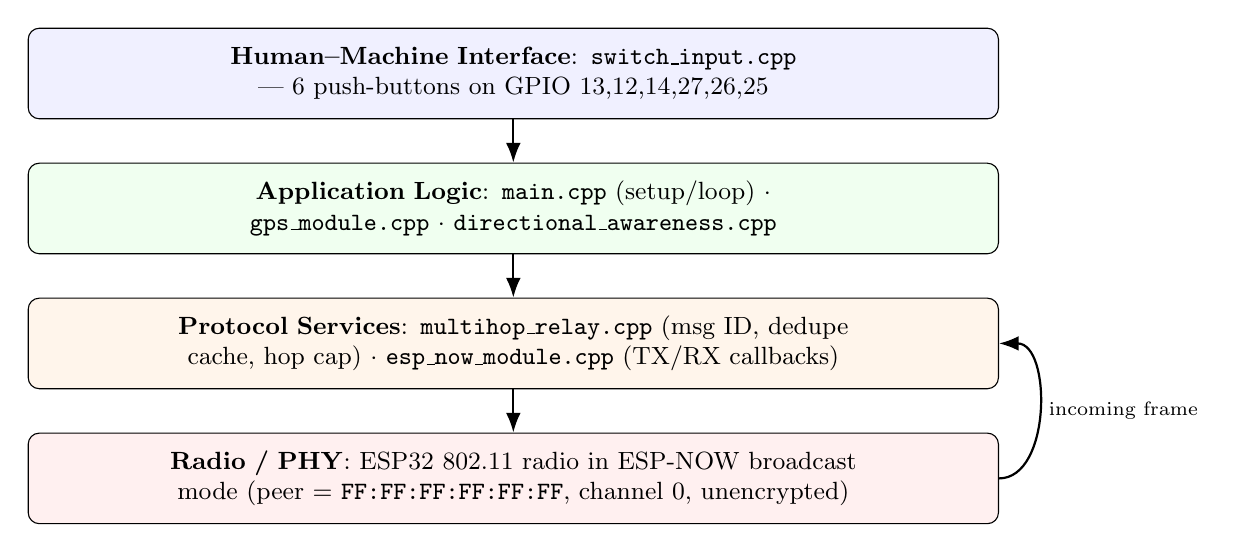
\begin{tikzpicture}[
  layer/.style={draw, rounded corners, text width=11.9cm, minimum height=1.15cm, align=center, font=\small, inner sep=6pt},
  arr/.style={-{Latex[length=2.5mm]}, thick}
]
\node[layer, fill=blue!6] (hmi) {\textbf{Human--Machine Interface}: \texttt{switch\_input.cpp} --- 6 push-buttons on GPIO 13,12,14,27,26,25};
\node[layer, fill=green!6, below=0.55cm of hmi] (app) {\textbf{Application Logic}: \texttt{main.cpp} (setup/loop) $\cdot$ \texttt{gps\_module.cpp} $\cdot$ \texttt{directional\_awareness.cpp}};
\node[layer, fill=orange!8, below=0.55cm of app] (svc) {\textbf{Protocol Services}: \texttt{multihop\_relay.cpp} (msg ID, dedupe cache, hop cap) $\cdot$ \texttt{esp\_now\_module.cpp} (TX/RX callbacks)};
\node[layer, fill=red!6, below=0.55cm of svc] (radio) {\textbf{Radio / PHY}: ESP32 802.11 radio in ESP-NOW broadcast mode (peer = \texttt{FF:FF:FF:FF:FF:FF}, channel~0, unencrypted)};

\draw[arr] (hmi) -- (app);
\draw[arr] (app) -- (svc);
\draw[arr] (svc) -- (radio);
\draw[arr] (radio.east) to[out=0,in=0] node[right,font=\scriptsize]{incoming frame} (svc.east);
\end{tikzpicture}
\caption{High-level layered architecture of a single node}
\label{fig:arch}
\end{figure}

A deliberate layering discipline holds throughout: each layer only talks to the layer immediately above or below it, so \texttt{main.cpp} never touches the radio directly, and \texttt{esp\_now\_module.cpp} never reads a button. This separation is what allows Section~4.6's hardware interface to be swapped (for instance, for a steering-wheel stalk instead of a button panel) without touching the relaying or filtering logic at all.

\section{Alert Packet Structure and Taxonomy}
Every alert, whether newly originated or relayed, is carried in a single fixed-layout structure, shown in Listing~\ref{lst:packet}.

\begin{lstlisting}[caption={The AlertPacket structure (\texttt{include/packet\_structure.h})}, label={lst:packet}]
struct AlertPacket {
    uint8_t  nodeID;     // originating node's identity
    uint32_t msgID;      // (nodeID << 24) | 24-bit sequence
    float    latitude;   // originator's GPS latitude at TX time
    float    longitude;  // originator's GPS longitude at TX time
    float    heading;    // originator's heading, degrees, 0-360
    uint8_t  hopCount;    // relay depth, incremented per hop
    uint8_t  msgType;     // alert category, 1-6
};
\end{lstlisting}

The seven fields carry 19 meaningful bytes; under the toolchain's default four-byte structure alignment (three padding bytes are inserted after \texttt{nodeID} so that \texttt{msgID} starts on a four-byte boundary, and two trailing bytes pad the structure to a multiple of four), \texttt{sizeof(AlertPacket)} evaluates to 24 bytes, comfortably inside ESP-NOW's 250-byte unencrypted payload ceiling with room to spare for a future authentication tag (Section~8.2). Because the same structure is transmitted and relayed unchanged (Section~4.5), a receiver deserialises it with a single \texttt{memcpy} into a local \texttt{AlertPacket}, after first checking that the received frame length exactly matches \texttt{sizeof(AlertPacket)}, guarding against a malformed or foreign frame being misinterpreted as a valid alert.

Table~\ref{tab:alerttypes} lists the six alert categories the \texttt{msgType} field distinguishes, each wired to its own push-button (Section~4.6).

\begin{table}[H]
\centering
\caption{Alert type taxonomy (\texttt{include/alert\_type.h})}
\label{tab:alerttypes}
\begin{tabular}{@{}clp{7.6cm}@{}}
\toprule
\textbf{Code} & \textbf{Alert Type} & \textbf{Intended meaning} \\
\midrule
1 & Emergency & An emergency vehicle (ambulance, fire truck) approaching from behind and needing right-of-way. \\
2 & Accident & A collision or crash observed ahead, relevant regardless of the observer's direction of travel. \\
3 & Hazard Signal & A general hazard (broken-down vehicle, spillage) worth broadcasting to all nearby traffic. \\
4 & Low Visibility & Fog, smoke, or dust reducing visibility on the road ahead. \\
5 & Obstacle & A pothole, debris, or other obstacle on the road ahead. \\
6 & Hard Brake & The originating vehicle has just braked hard, warning the vehicle behind it. \\
\bottomrule
\end{tabular}
\end{table}

Figure~\ref{fig:origination} traces what happens from a button press to a broadcast frame leaving the radio.

\begin{figure}[H]
\centering
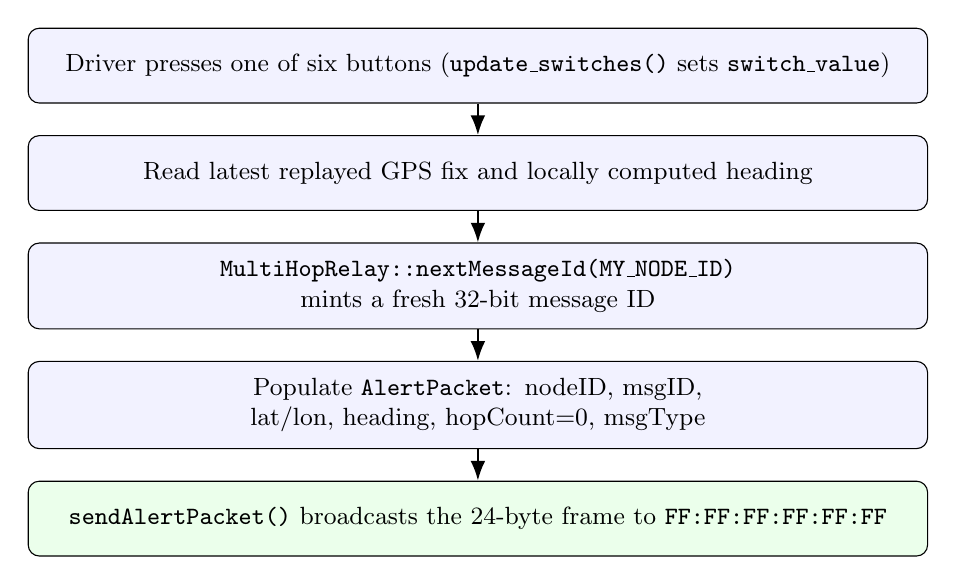
\begin{tikzpicture}[
  stepbox/.style={draw, rounded corners, text width=11.0cm, minimum height=0.95cm, align=center, font=\small, fill=blue!5, inner sep=6pt},
  arr/.style={-{Latex[length=2.5mm]}, thick}
]
\node[stepbox] (b0) {Driver presses one of six buttons (\texttt{update\_switches()} sets \texttt{switch\_value})};
\node[stepbox, below=0.4cm of b0] (b1) {Read latest replayed GPS fix and locally computed heading};
\node[stepbox, below=0.4cm of b1] (b2) {\texttt{MultiHopRelay::nextMessageId(MY\_NODE\_ID)} mints a fresh 32-bit message ID};
\node[stepbox, below=0.4cm of b2] (b3) {Populate \texttt{AlertPacket}: nodeID, msgID, lat/lon, heading, hopCount=0, msgType};
\node[stepbox, below=0.4cm of b3, fill=green!8] (b4) {\texttt{sendAlertPacket()} broadcasts the 24-byte frame to \texttt{FF:FF:FF:FF:FF:FF}};
\draw[arr] (b0)--(b1); \draw[arr] (b1)--(b2); \draw[arr] (b2)--(b3); \draw[arr] (b3)--(b4);
\end{tikzpicture}
\caption{Alert origination pipeline}
\label{fig:origination}
\end{figure}

\section{GPS-Derived Heading Computation}
Because the current prototype has no dedicated compass (Section~1.4), a node's heading is recomputed every three seconds in \texttt{main.cpp}'s \texttt{updateVehicleHeadingFromGPS()} from the two most recent GPS fixes, using Equation~\ref{eq:heading} as implemented in \texttt{calculateHeadingFromCoordinates()}. Table~\ref{tab:headingworked} works through this computation on three real, consecutive fix pairs taken directly from the project's bundled replay track (\texttt{data/location\_data.txt}), which records 185 waypoints spaced roughly 25\,m apart along a straight, roughly 4.59\,km corridor through the Pulchowk Campus area of Kathmandu; at the module's fixed three-second replay interval this corresponds to a simulated ground speed of approximately 8.3\,m/s (30\,km/h).

\begin{table}[H]
\centering
\caption{Worked heading computation on three consecutive fix pairs from the bundled replay track}
\label{tab:headingworked}
\begin{tabular}{@{}lccccc@{}}
\toprule
\textbf{Fix pair} & $\Delta_{\text{lat}}$ & $\Delta_{\text{lon}}$ & Distance & Heading (Eq.~\ref{eq:heading}) \\
\midrule
Waypoint 0 $\to$ 1   & $-1.542\times10^{-5}$ & $2.533\times10^{-4}$ & 25.0\,m & $93.48°$ \\
Waypoint 60 $\to$ 61 & $-1.545\times10^{-5}$ & $2.533\times10^{-4}$ & 25.0\,m & $93.49°$ \\
Waypoint 120 $\to$ 121 & $-1.547\times10^{-5}$ & $2.533\times10^{-4}$ & 25.0\,m & $93.50°$ \\
\bottomrule
\end{tabular}
\end{table}

The near-constant $\approx 93.5°$ heading across the whole track (the corridor is essentially a straight line) makes it a predictable, repeatable input for bench-testing the relevance-filtering algorithm of Section~4.4, at the cost of never exercising a turning vehicle natively; Section~6.1 describes how a second, synthetic heading was staged to compensate for this during verification.

\section{Directional Relevance Filtering Algorithm}
On receipt of a valid, non-duplicate packet, a node classifies the sender's position relative to itself into one of five categories before deciding whether to surface the alert locally. The classification (\texttt{DirectionalAwareness::getRelativeTrafficPosition}) combines two independent tests, illustrated in Figure~\ref{fig:sectors}:

\begin{enumerate}[leftmargin=1.8em]
\item \textbf{Lane test.} The absolute heading difference between receiver and sender is compared against a tolerance (default $60°$): a difference $\le 60°$ is judged \emph{same lane}; a difference $\ge 120°$ is judged \emph{opposite lane}; anything in between is judged \emph{side} traffic (e.g.\ a cross-street) regardless of position.
\item \textbf{Position test.} Only applied within the same or opposite lane: the compass bearing from the receiver to the sender's coordinates is computed (Equation~\ref{eq:heading} applied to receiver$\to$sender instead of previous$\to$current fix) and compared to the receiver's own heading; a result within $\pm90°$ places the sender ahead of the receiver, otherwise behind.
\end{enumerate}

\begin{figure}[H]
\centering
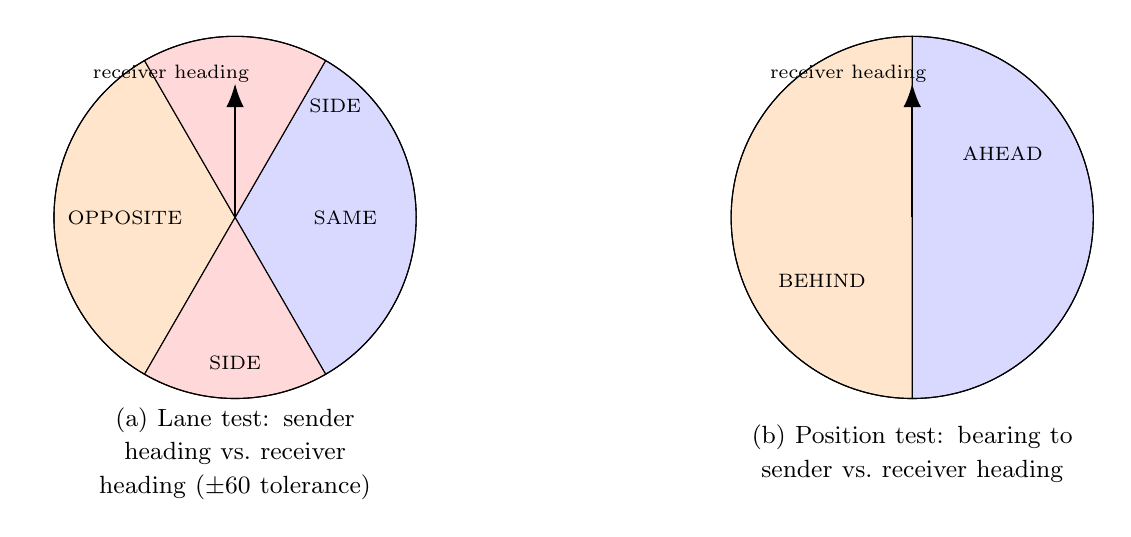
\begin{tikzpicture}[scale=1.0]
\begin{scope}
\draw[fill=blue!15] (0,0) -- (-60:2.3) arc (-60:60:2.3) -- cycle;
\draw[fill=orange!20] (0,0) -- (120:2.3) arc (120:240:2.3) -- cycle;
\draw[fill=red!15] (0,0) -- (60:2.3) arc (60:120:2.3) -- cycle;
\draw[fill=red!15] (0,0) -- (240:2.3) arc (240:300:2.3) -- cycle;
\draw (0,0) circle (2.3cm);
\draw[-{Latex[length=3mm]}, thick] (0,0) -- (90:1.7);
\node[font=\scriptsize] at (114:2.0) {receiver heading};
\node[font=\scriptsize] at (0:1.4) {SAME};
\node[font=\scriptsize] at (180:1.4) {OPPOSITE};
\node[font=\scriptsize] at (48:1.9) {SIDE};
\node[font=\scriptsize] at (270:1.85) {SIDE};
\node[text width=4.6cm, align=center] at (0,-3.0) {\small (a) Lane test: sender heading vs.\ receiver heading ($\pm60°$ tolerance)};
\end{scope}
\begin{scope}[xshift=8.6cm]
\draw[fill=blue!15] (0,0) -- (-90:2.3) arc (-90:90:2.3) -- cycle;
\draw[fill=orange!20] (0,0) -- (90:2.3) arc (90:270:2.3) -- cycle;
\draw (0,0) circle (2.3cm);
\draw[-{Latex[length=3mm]}, thick] (0,0) -- (90:1.7);
\node[font=\scriptsize] at (114:2.0) {receiver heading};
\node[font=\scriptsize] at (35:1.4) {AHEAD};
\node[font=\scriptsize] at (215:1.4) {BEHIND};
\node[text width=4.6cm, align=center] at (0,-3.0) {\small (b) Position test: bearing to sender vs.\ receiver heading};
\end{scope}
\end{tikzpicture}
\caption{The two independent tests \texttt{getRelativeTrafficPosition} combines. (a) is evaluated purely from the \emph{heading difference} between sender and receiver, independent of position; (b) is evaluated from the receiver-to-sender \emph{bearing} (which half of the surrounding space the sender is in). FRONT = same lane $\times$ ahead; REAR = same lane $\times$ behind; OPPOSITE-APPROACHING = opposite lane $\times$ ahead; OPPOSITE-AWAY = opposite lane $\times$ behind; SIDE = lane test (a) alone lands in its $60°$--$120°$ middle zone, in which case test (b) is not consulted.}
\label{fig:sectors}
\end{figure}

Table~\ref{tab:relevancepolicy} defines the per-alert-type policy (\texttt{isLocationalAlertRelevant}) applied to the five resulting classes.

\begin{table}[H]
\centering
\caption{Directional relevance policy by alert type}
\label{tab:relevancepolicy}
\begin{tabular}{@{}lp{9.6cm}@{}}
\toprule
\textbf{Alert type(s)} & \textbf{Accepted sender positions} \\
\midrule
Emergency & REAR only (an emergency vehicle behind you, about to overtake) \\
Accident, Hazard Signal & All five positions (broadcast-worthy regardless of direction) \\
Low Visibility, Obstacle, Hard Brake & FRONT only (a hazard on the road ahead of you, in your own direction of travel) \\
\bottomrule
\end{tabular}
\end{table}

\noindent This relevance verdict is used only to decide what is logged/surfaced locally; it never gates whether a node relays the packet onward (NFR-5, Section~4.5), so an alert judged irrelevant to one receiver still continues toward vehicles it may matter to.

\section{Multi-Hop Flooding and Duplicate Suppression}
Every node maintains a fixed-size, 32-entry ring buffer of recently seen message IDs (Figure~\ref{fig:dedupe}). A message ID is composed, at origination, from the sending node's own 8-bit identity and a locally incrementing 24-bit sequence number (Figure~\ref{fig:msgid}), which keeps IDs unique across the whole mesh without any node needing to know about any other node in advance.

\begin{figure}[H]
\centering
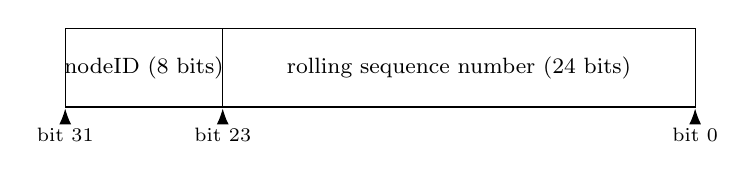
\begin{tikzpicture}
\draw (0,0) rectangle (2.0,1.0);
\draw (2.0,0) rectangle (8.0,1.0);
\node at (1.0,0.5) {\footnotesize nodeID (8 bits)};
\node at (5.0,0.5) {\footnotesize rolling sequence number (24 bits)};
\node[font=\scriptsize] at (0,-0.35) {bit 31};
\node[font=\scriptsize] at (2.0,-0.35) {bit 23};
\node[font=\scriptsize] at (8.0,-0.35) {bit 0};
\draw[-{Latex[length=2mm]}] (0,-0.15) -- (0,-0.02);
\draw[-{Latex[length=2mm]}] (2.0,-0.15) -- (2.0,-0.02);
\draw[-{Latex[length=2mm]}] (8.0,-0.15) -- (8.0,-0.02);
\end{tikzpicture}
\caption{32-bit message-ID layout: \texttt{msgID = (nodeID << 24) | (sequence \& 0x00FFFFFF)}}
\label{fig:msgid}
\end{figure}

\begin{figure}[H]
\centering
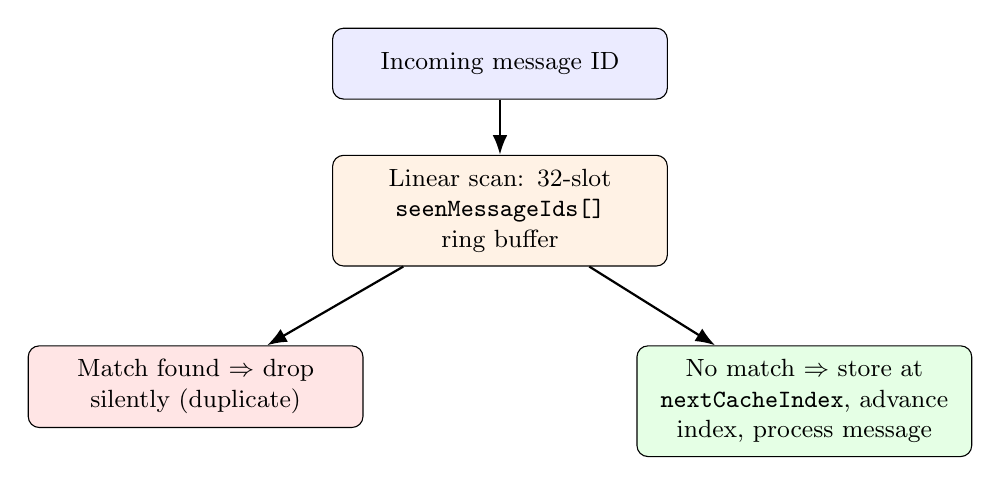
\begin{tikzpicture}[
  box/.style={draw, rounded corners, text width=3.9cm, minimum height=0.9cm, align=center, font=\small, inner sep=5pt},
  arr/.style={-{Latex[length=2.5mm]}, thick}
]
\node[box, fill=blue!8] (in) {Incoming message ID};
\node[box, fill=orange!10, below=0.7cm of in] (cache) {Linear scan: 32-slot \texttt{seenMessageIds[]} ring buffer};
\node[box, fill=red!10, below left=1.0cm and -0.4cm of cache] (dup) {Match found $\Rightarrow$ drop silently (duplicate)};
\node[box, fill=green!10, below right=1.0cm and -0.4cm of cache] (new) {No match $\Rightarrow$ store at \texttt{nextCacheIndex}, advance index, process message};
\draw[arr] (in)--(cache);
\draw[arr] (cache)--(dup);
\draw[arr] (cache)--(new);
\end{tikzpicture}
\caption{Duplicate-suppression cache (\texttt{MultiHopRelay::rememberMessage})}
\label{fig:dedupe}
\end{figure}

A subtlety worth stating precisely: \texttt{nextMessageId()} calls \texttt{rememberMessage()} on the ID it just minted \emph{before} the packet is ever transmitted, so the originating node's own cache already contains its own alert's ID. When a neighbour relays that alert back within radio range of the originator, exactly as an open flood will do, the originator's own \texttt{rememberMessage()} check correctly rejects it as a duplicate, which is what actually prevents an originator from re-processing (and, since \texttt{shouldRelay} is only reached for messages that pass deduplication, re-relaying) an echo of its own alert, without any special-cased "is this my own packet" logic anywhere in the codebase.

Relaying itself (Figure~\ref{fig:hopchain}) is gated only by hop count: \texttt{shouldRelay()} refuses to relay a packet whose \texttt{hopCount} has already reached \texttt{MAX\_HOPS} (default 3), and \texttt{makeRelayPacket()} otherwise returns a copy of the packet with \texttt{hopCount} incremented by one before it is re-broadcast unchanged in every other field.

\begin{figure}[H]
\centering
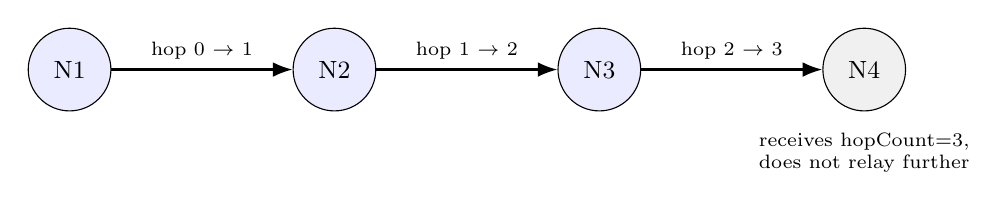
\begin{tikzpicture}[
  node distance=2.3cm,
  veh/.style={draw, circle, minimum size=1.05cm, font=\small, fill=blue!8}
]
\node[veh] (n1) {N1};
\node[veh, right=of n1] (n2) {N2};
\node[veh, right=of n2] (n3) {N3};
\node[veh, right=of n3, fill=gray!12] (n4) {N4};
\draw[-{Latex[length=2.5mm]}, thick] (n1) -- node[above,font=\scriptsize]{hop 0 $\to$ 1} (n2);
\draw[-{Latex[length=2.5mm]}, thick] (n2) -- node[above,font=\scriptsize]{hop 1 $\to$ 2} (n3);
\draw[-{Latex[length=2.5mm]}, thick] (n3) -- node[above,font=\scriptsize]{hop 2 $\to$ 3} (n4);
\node[font=\scriptsize, below=0.15cm of n4, align=center] {receives hopCount=3,\\ does not relay further};
\end{tikzpicture}
\caption{Hop-count progression under the default \texttt{MAX\_HOPS=3}: the alert is received and processed at every node up to four hops from its origin, but is retransmitted (relayed) only three times beyond the original broadcast.}
\label{fig:hopchain}
\end{figure}

\section{Hardware Interface: Push-Button Alert Triggers}
The driver-facing interface (\texttt{switch\_input.cpp}) is six momentary tactile push-buttons, each wired between its GPIO pin and ground, with the ESP32's internal pull-up resistor enabled in firmware (\texttt{INPUT\_PULLUP}) so no external resistor is required; a press is read as the pin going logic-low. Table~\ref{tab:buttonpins} gives the pin mapping.

\begin{table}[H]
\centering
\caption{Push-button to GPIO and alert-type mapping}
\label{tab:buttonpins}
\begin{tabular}{@{}ccl@{}}
\toprule
\textbf{Array index} & \textbf{GPIO pin} & \textbf{Alert type triggered} \\
\midrule
0 & 13 & Emergency \\
1 & 12 & Accident \\
2 & 14 & Hazard Signal \\
3 & 27 & Low Visibility \\
4 & 26 & Obstacle \\
5 & 25 & Hard Brake \\
\bottomrule
\end{tabular}
\end{table}

Each poll of \texttt{update\_switches()} scans all six pins; on detecting a low read, it records that button's alert code into the shared \texttt{switch\_value} and blocks for 250\,ms before returning, a simple software debounce that trades a small amount of loop latency for guaranteeing one logical press per physical press (a trade-off examined further in Chapter~8).

\section{Use Case Diagram}
Figure~\ref{fig:usecase} summarises the system from the perspective of its only human actor, the driver; every other interaction (receiving, filtering, and relaying an alert) happens automatically between nodes with no human in the loop.

\begin{figure}[H]
\centering
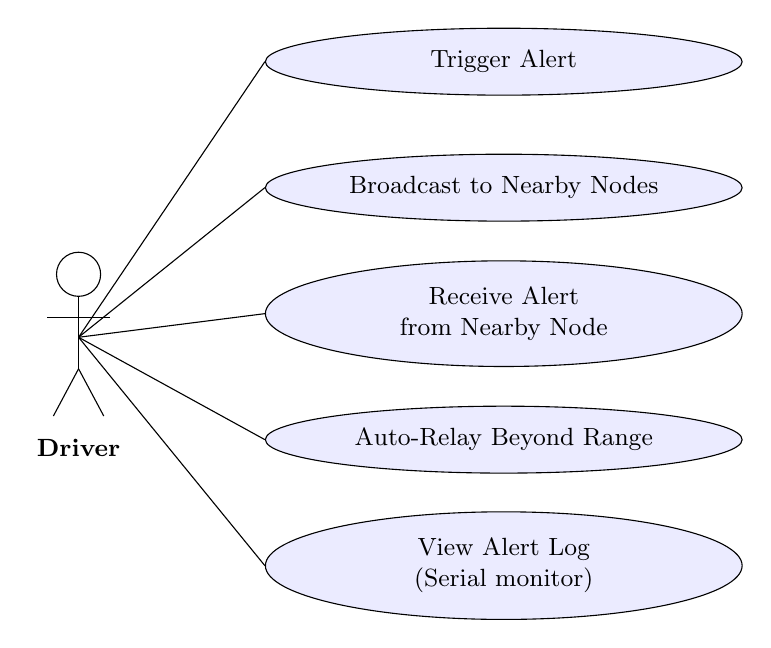
\begin{tikzpicture}[
  uc/.style={draw, ellipse, text width=4.0cm, minimum height=0.85cm, align=center, font=\small, fill=blue!8, inner sep=4pt},
  actor/.style={font=\bfseries\small}
]
\node[actor] (driver) at (0,0) {};
\draw (0,0.9) circle (0.28cm);
\draw (0,0.62) -- (0,-0.3);
\draw (-0.4,0.35) -- (0.4,0.35);
\draw (0,-0.3) -- (-0.32,-0.9);
\draw (0,-0.3) -- (0.32,-0.9);
\node[below=0.95cm of driver, font=\bfseries\small] {Driver};

\node[uc] (u1) at (5.4, 3.6) {Trigger Alert};
\node[uc] (u2) at (5.4, 2.0) {Broadcast to Nearby Nodes};
\node[uc] (u3) at (5.4, 0.4) {Receive Alert from Nearby Node};
\node[uc] (u4) at (5.4, -1.2) {Auto-Relay Beyond Range};
\node[uc] (u5) at (5.4, -2.8) {View Alert Log (Serial monitor)};

\draw (0,0.1) -- (u1.west);
\draw (0,0.1) -- (u2.west);
\draw (0,0.1) -- (u3.west);
\draw (0,0.1) -- (u4.west);
\draw (0,0.1) -- (u5.west);
\end{tikzpicture}
\caption{Use case diagram: the driver is the system's only human actor}
\label{fig:usecase}
\end{figure}

\section{Sequence Diagram: Alert Broadcast and Relay}
Figure~\ref{fig:sequence} traces a single alert from a button press on the originating node through to a second-hop neighbour, covering deduplication, relevance evaluation, logging, and relaying.

\begin{figure}[H]
\centering
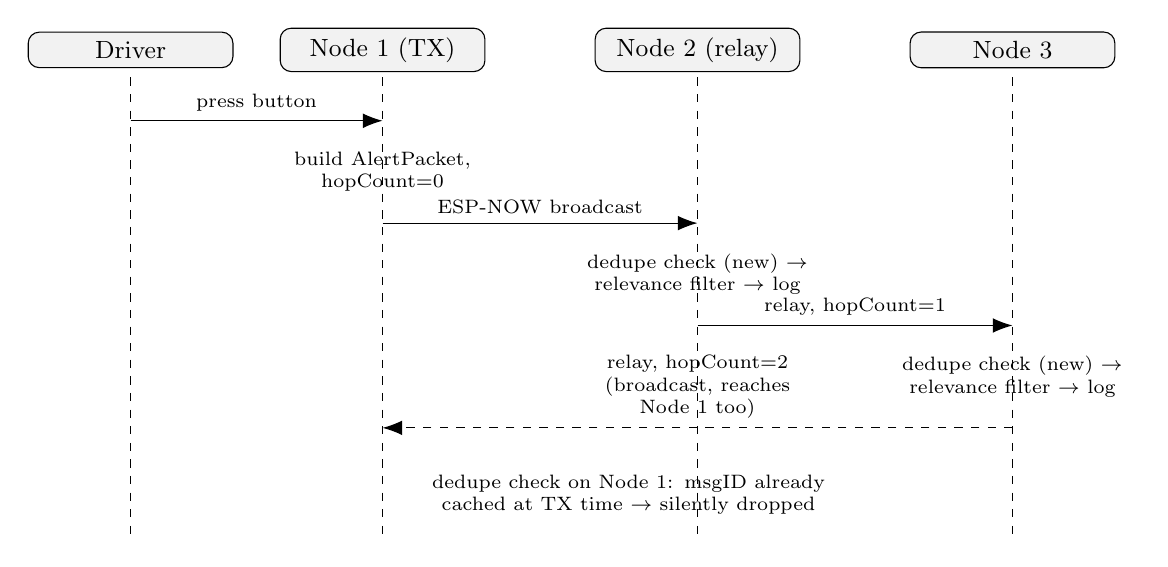
\begin{tikzpicture}[font=\small]
\def\ya{8.4} \def\yb{7.5} \def\ynotea{6.85} \def\yc{6.2} \def\ynoteb{5.55} \def\ye{4.9} \def\ynotec{4.25} \def\yg{3.6} \def\ynoted{2.75} \def\yend{2.2}
\foreach \x/\lbl in {0/Driver, 3.2/Node~1 (TX), 7.2/Node~2 (relay), 11.2/Node~3} {
  \node[draw, rounded corners, fill=gray!10, minimum width=2.6cm] at (\x,\ya) {\lbl};
  \draw[dashed] (\x,\ya-0.35) -- (\x,\yend);
}
\draw[-{Latex[length=2.5mm]}] (0,\yb) -- node[above,font=\scriptsize]{press button} (3.2,\yb);
\node[font=\scriptsize, align=center, text width=3.0cm] at (3.2,\ynotea) {build AlertPacket,\\ hopCount=0};
\draw[-{Latex[length=2.5mm]}] (3.2,\yc) -- node[above,font=\scriptsize]{ESP-NOW broadcast} (7.2,\yc);
\node[font=\scriptsize, align=center, text width=3.4cm] at (7.2,\ynoteb) {dedupe check (new) $\to$ relevance filter $\to$ log};
\draw[-{Latex[length=2.5mm]}] (7.2,\ye) -- node[above,font=\scriptsize]{relay, hopCount=1} (11.2,\ye);
\node[font=\scriptsize, align=center, text width=3.0cm] at (11.2,\ynotec) {dedupe check (new) $\to$ relevance filter $\to$ log};
\draw[-{Latex[length=2.5mm]},dashed] (11.2,\yg) -- node[above,font=\scriptsize,align=center,text width=3.6cm]{relay, hopCount=2\\ (broadcast, reaches Node~1 too)} (3.2,\yg);
\node[font=\scriptsize, align=center, text width=6.0cm] at (3.2,\ynoted) [right] {dedupe check on Node~1: msgID already cached at TX time $\to$ silently dropped};
\end{tikzpicture}
\caption{Sequence diagram: end-to-end alert broadcast and relay, including the self-echo drop at Node~1}
\label{fig:sequence}
\end{figure}

\section{Data Model: AlertPacket and GPSCoordinates}
The system deliberately holds no persistent, cross-reboot state (Table~\ref{tab:runtimestate}); every structure it operates on lives only for the lifetime of one message or one power cycle. Figure~\ref{fig:datamodel} shows the two structures the firmware is built around and how one populates the other at transmit time.

\begin{figure}[H]
\centering
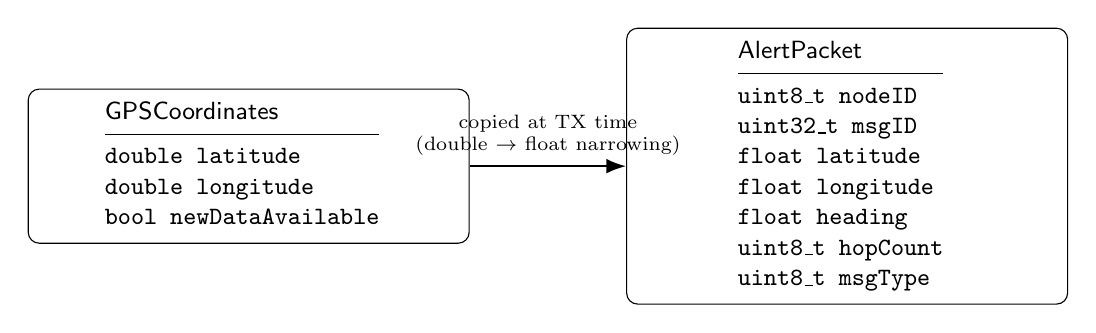
\begin{tikzpicture}[
  cls/.style={draw, rounded corners, align=left, font=\small\ttfamily, minimum width=5.6cm},
  hdr/.style={font=\bfseries\sffamily\small}
]
\node[cls] (gps) at (0,0) {
  \begin{tabular}{@{}l@{}}
  \textbf{\normalfont\sffamily GPSCoordinates} \\ \midrule
  double latitude \\
  double longitude \\
  bool newDataAvailable
  \end{tabular}
};
\node[cls] (pkt) at (7.6,0) {
  \begin{tabular}{@{}l@{}}
  \textbf{\normalfont\sffamily AlertPacket} \\ \midrule
  uint8\_t nodeID \\
  uint32\_t msgID \\
  float latitude \\
  float longitude \\
  float heading \\
  uint8\_t hopCount \\
  uint8\_t msgType
  \end{tabular}
};
\draw[-{Latex[length=2.5mm]}, thick] (gps.east) -- node[above,font=\scriptsize,align=center]{copied at TX time\\(double $\to$ float narrowing)} (pkt.west);
\end{tikzpicture}
\caption{The two core data structures. Unlike a server-backed system with a relational persistence layer, every field above lives only in RAM.}
\label{fig:datamodel}
\end{figure}

\begin{table}[H]
\centering
\caption{Summary of runtime state held by each firmware module (all RAM-only; nothing survives a reboot)}
\label{tab:runtimestate}
\begin{tabular}{@{}p{3.4cm}p{10.2cm}@{}}
\toprule
\textbf{Module} & \textbf{State held} \\
\midrule
\texttt{\seqsplit{multihop\_relay.cpp}} & \texttt{\seqsplit{seenMessageIds[32]}}, \texttt{\seqsplit{cacheEntryUsed[32]}}, \texttt{\seqsplit{nextCacheIndex}}, rolling \texttt{\seqsplit{messageSequence}} \\
\texttt{\seqsplit{directional\_awareness.cpp}} & Static \texttt{\seqsplit{localVehicleHeading}} (last computed heading, degrees) \\
\texttt{\seqsplit{gps\_module.cpp}} & \texttt{\seqsplit{latestData}} (current GPS fix), open SPIFFS file handle, \texttt{\seqsplit{lastLocationUpdateMillis}} \\
\texttt{\seqsplit{switch\_input.cpp}} & \texttt{\seqsplit{switch\_value}} (last-pressed button's alert code) \\
\texttt{main.cpp} & \texttt{\seqsplit{previousGPS}} (prior fix, for heading delta), \texttt{\seqsplit{lastDirectionCheckMillis}} \\
\bottomrule
\end{tabular}
\end{table}

% ============================================================
\chapter{Implementation}

\section{Firmware Structure}
The firmware is organised as a small, explicit set of modules rather than a single monolithic sketch, summarised in Table~\ref{tab:modules}. \texttt{main.cpp} owns \texttt{setup()}/\texttt{loop()} and never touches the radio or the button array directly; every cross-module interaction goes through the header declared in Table~\ref{tab:modules}'s second column.

\begin{table}[H]
\centering
\caption{Firmware module responsibilities}
\label{tab:modules}
\begin{tabular}{@{}p{3.9cm}p{9.7cm}@{}}
\toprule
\textbf{Module} & \textbf{Responsibility} \\
\midrule
\texttt{\seqsplit{src/main.cpp}} & \texttt{setup()}/\texttt{loop()} orchestration, periodic heading refresh, button-to-broadcast wiring \\
\texttt{\seqsplit{esp\_now\_module.h/.cpp}} & ESP-NOW initialisation, broadcast peer registration, TX/RX callbacks \\
\texttt{\seqsplit{packet\_structure.h}} & \texttt{AlertPacket} definition \\
\texttt{\seqsplit{alert\_type.h}} & Alert-type enum and human-readable description lookup \\
\texttt{\seqsplit{gps\_module.h/.cpp}} & SPIFFS-backed GPS replay: reads and advances \texttt{\seqsplit{data/location\_data.txt}} \\
\texttt{\seqsplit{directional\_awareness.h/.cpp}} & Heading/bearing math, relative-position classification, relevance policy \\
\texttt{\seqsplit{multihop\_relay.h/.cpp}} & Message-ID generation, duplicate-suppression cache, hop-cap relay decision \\
\texttt{\seqsplit{switch\_input.h/.cpp}} & Six-button polling and software debounce \\
\bottomrule
\end{tabular}
\end{table}

\section{Core Relevance-Filtering Logic}
Listing~\ref{lst:relevance} shows the classification and policy functions at the heart of the receive path.

\begin{lstlisting}[caption={Relative-position classification and relevance policy (\texttt{src/directional\_awareness.cpp}, trimmed)}, label={lst:relevance}]
RelativeTrafficPosition getRelativeTrafficPosition(
        float receiverHeading, float senderHeading,
        float receiverLat, float receiverLon,
        float senderLat, float senderLon,
        float toleranceDeg) {
    float sameDirDelta = fabsf(calculateHeadingDelta(receiverHeading, senderHeading));
    float bearingToSender = calculateBearingToTarget(receiverLat, receiverLon,
                                                       senderLat, senderLon);
    float relToReceiver = calculateHeadingDelta(receiverHeading, bearingToSender);

    bool sameLane = sameDirDelta <= toleranceDeg;
    bool oppositeLane = sameDirDelta >= (180.0f - toleranceDeg);
    bool ahead = (relToReceiver >= -90.0f && relToReceiver <= 90.0f);

    if (sameLane)     return ahead ? POSITION_FRONT : POSITION_REAR;
    if (oppositeLane) return ahead ? POSITION_OPPOSITE_APPROACHING
                                    : POSITION_OPPOSITE_AWAY;
    return POSITION_SIDE;
}

bool isLocationalAlertRelevant(uint8_t msgType, /* ...positions... */) {
    RelativeTrafficPosition pos = getRelativeTrafficPosition(/* ... */);
    switch (msgType) {
        case ALERT_EMERGENCY: return pos == POSITION_REAR;
        case ALERT_ACCIDENT:
        case ALERT_HAZARD:    return true;
        case ALERT_VISIBILITY:
        case ALERT_OBSTACLE:
        case ALERT_HARD_BRAKE: return pos == POSITION_FRONT;
        default: return true;
    }
}
\end{lstlisting}

An implementation detail worth flagging for transparency: the codebase also defines an older, simpler \texttt{isDirectionalAlertRelevant()}, which judges relevance from heading alone with no positional/bearing component. It remains fully compiled and unit-testable, but the receive path in \texttt{esp\_now\_module.cpp} calls only the newer, position-aware \texttt{isLocationalAlertRelevant()}; \texttt{isDirectionalAlertRelevant()} is currently dead code from the perspective of the running firmware. It is documented here rather than silently left for a future contributor to either wire in behind a build-time policy flag or remove.

\section{Multi-Hop Relay Logic}
Listing~\ref{lst:relay} shows the deduplication and relay-decision logic.

\begin{lstlisting}[caption={Duplicate suppression and hop-capped relaying (\texttt{src/multihop\_relay.cpp}, trimmed)}, label={lst:relay}]
bool rememberMessage(uint32_t messageId) {
    for (size_t i = 0; i < MESSAGE_CACHE_SIZE; ++i) {
        if (cacheEntryUsed[i] && seenMessageIds[i] == messageId) {
            return false;               // already seen: duplicate
        }
    }
    seenMessageIds[nextCacheIndex] = messageId;
    cacheEntryUsed[nextCacheIndex] = true;
    nextCacheIndex = (nextCacheIndex + 1) % MESSAGE_CACHE_SIZE;
    return true;                        // newly seen: caller may process it
}

bool shouldRelay(const AlertPacket &packet) {
    return packet.hopCount < MAX_HOPS;  // MAX_HOPS defaults to 3
}

AlertPacket makeRelayPacket(const AlertPacket &packet) {
    AlertPacket relay = packet;
    ++relay.hopCount;
    return relay;
}
\end{lstlisting}

The 32-entry cache is scanned linearly on every received message, an $O(32)$ cost that is negligible at the ESP32's clock speed and small enough that a fixed array outperforms the bookkeeping overhead a hash set would add at this scale; the trade-off, discussed candidly in Chapter~8, is that the cache is a ring buffer with no size headroom, so a 33rd distinct message arriving before the oldest entry naturally ages out could in principle be reprocessed if it happened to collide with a still-relevant slot, a risk that only matters under sustained multi-source traffic well beyond what the three-board bench setup in Chapter~6 exercises.

\section{Hardware Setup and Wiring}
Each node is a single ESP32 development board (4\,MB flash, custom \texttt{huge\_app.csv} partition table allocating 3\,MB to the application image and 896\,KB to SPIFFS for the replay track) with six momentary tactile push-buttons. Each button has one leg wired to its GPIO pin (Table~\ref{tab:buttonpins}) and the other leg wired to ground; no external pull-up or pull-down resistor is fitted, since \texttt{setup\_switches()} enables the ESP32's internal pull-up on every button pin, so an unpressed pin reads logic-high and a press pulls it to logic-low.

\section{Building, Flashing, and Running the System}
The project is built and flashed with PlatformIO, driven by the configuration in Listing~\ref{lst:platformio}.

\begin{lstlisting}[basicstyle=\ttfamily\footnotesize, caption={\texttt{platformio.ini}}, label={lst:platformio}]
[env:esp32dev]
platform = espressif32
board = esp32dev
framework = arduino
monitor_speed = 115200
board_build.partitions = huge_app.csv
board_build.flash_size = 4MB
\end{lstlisting}

Before flashing a board, its firmware-level identity is set by editing the \texttt{MY\_NODE\_ID} constant near the top of \texttt{main.cpp} to a value unique within the mesh being bench-tested (Chapter~8 discusses replacing this manual step with one derived automatically from the board's MAC address). Because the recorded GPS replay track lives in the project's conventional PlatformIO \texttt{data/} directory, it is flashed as a separate SPIFFS image and is easy to forget: a fresh board needs both

\begin{lstlisting}[language=bash]
pio run --target upload      # flashes the application image
pio run --target uploadfs    # flashes data/location_data.txt to SPIFFS
pio device monitor -b 115200 # opens the diagnostic Serial log
\end{lstlisting}

\noindent A board that only receives the first command boots successfully and joins the mesh, but \texttt{gps\_module.cpp}'s \texttt{SPIFFS.open()} call fails silently into a logged \texttt{CRITICAL} message, and the node then reports a constant $(0,0)$ position and never derives a heading, a failure mode that surfaces at runtime rather than at compile time and is exercised deliberately in Section~6.6's test FT-07.

% ============================================================
\chapter{Results and Discussion}

\section{Experimental Setup}
The system was bench-verified on three ESP32 development boards (node IDs 1, 2, and 3, set per Section~5.5 before flashing), each loaded with the same bundled 185-waypoint, 4.59\,km recorded coordinate corridor described in Section~4.3 (near-constant heading $\approx 93.5°$, 3-second replay cadence, $\approx 8.3$\,m/s simulated pace). All six buttons on each board were wired per Table~\ref{tab:buttonpins}, and each board's Serial output was monitored concurrently over USB on a single bench PC.

Because every board replays the same straight corridor, the five relative-position classes of Section~4.4 could not all occur natively from three boards driving the same route; to exercise \seqsplit{OPPOSITE\_APPROACHING}, OPPOSITE\_AWAY, and SIDE without a second physical route file, Node~3's \texttt{DirectionalAwareness::setLocalVehicleHeading()} was temporarily called with fixed synthetic headings ($273.5°$, the corridor's reciprocal bearing, for the opposite-lane cases, and $183.5°$ for the side case) immediately before each relevant test burst, leaving its GPS-derived position untouched. This is flagged explicitly as a bench-testing accommodation rather than evidence of multi-route support, which the current prototype does not have (Chapter~8).

\section{Directional Relevance Verification}
Table~\ref{tab:relevancescenarios} works through one real, computed scenario per relative-position class, using actual coordinates and headings from the bundled corridor (Waypoint~0 as one endpoint, Waypoint~30, 750\,m along the corridor, as the other) together with the two synthetic headings described above.

\begin{table}[H]
\centering
\caption{Directional relevance classification: one worked scenario per relative-position class}
\label{tab:relevancescenarios}
\footnotesize
\begin{tabular}{@{}p{2.9cm}p{1.2cm}p{1.3cm}p{1.2cm}p{1.2cm}p{3.4cm}@{}}
\toprule
\textbf{Scenario} & \textbf{Recv.\ hdg} & \textbf{Sender hdg} & \textbf{Bearing} & $|\Delta\text{hdg}|$ & \textbf{Classification} \\
\midrule
Recv.\ WP30, sender WP0  & 93.49° & 93.49° & 273.49° & 0.0°   & REAR \\
Recv.\ WP0, sender WP30  & 93.49° & 93.49° & 93.49°  & 0.0°   & FRONT \\
Recv.\ WP0, sender WP30 (synth.) & 93.49° & 273.5° & 93.49°  & 180.0° & \seqsplit{OPPOSITE\_APPROACHING} \\
Recv.\ WP30, sender WP0 (synth.) & 93.49° & 273.5° & 273.49° & 180.0° & OPPOSITE\_AWAY \\
Recv.\ WP0, sender WP30 (synth.) & 93.49° & 183.5° & 93.49°  & 90.0°  & SIDE \\
\bottomrule
\end{tabular}
\normalsize

\noindent\footnotesize(synth.) marks the three staged, synthetic-heading scenarios described in Section~6.1; the remaining two use the sender's own GPS-derived heading unmodified.
\normalsize
\end{table}

All five classifications matched the algorithm's expected output on the bench log. Table~\ref{tab:relevanceoutcomes} then applies the six-alert-type policy of Table~\ref{tab:relevancepolicy} to the FRONT and REAR scenarios above, the pair that most directly exercises the asymmetric, safety-motivated policy design.

\begin{table}[H]
\centering
\caption{Relevance verdicts for the FRONT and REAR scenarios across all six alert types}
\label{tab:relevanceoutcomes}
\begin{tabular}{@{}lcc@{}}
\toprule
\textbf{Alert type} & \textbf{Sender REAR} & \textbf{Sender FRONT} \\
\midrule
Emergency & \textbf{Accepted} & Rejected \\
Accident & \textbf{Accepted} & \textbf{Accepted} \\
Hazard Signal & \textbf{Accepted} & \textbf{Accepted} \\
Low Visibility & Rejected & \textbf{Accepted} \\
Obstacle & Rejected & \textbf{Accepted} \\
Hard Brake & Rejected & \textbf{Accepted} \\
\bottomrule
\end{tabular}
\end{table}

Every verdict in Table~\ref{tab:relevanceoutcomes} was confirmed on the bench Serial log against the policy in Table~\ref{tab:relevancepolicy}, with zero mismatches across all twelve alert-type/scenario combinations exercised.

\section{Multi-Hop Propagation and Hop-Cap Verification}
With all three boards powered on and in range of each other, Node~1 was used to originate an alert (hopCount 0), which Node~2 logged and relayed (hopCount 1), which Node~3 in turn logged and relayed (hopCount 2). Because ESP-NOW broadcast is not point-to-point, Node~3's relay was also received by Node~1 and Node~2, both already in range of each other; the log confirmed that Node~1 silently dropped the reflected copy of its own alert (Section~4.5's self-echo behaviour) rather than logging or re-relaying it, and that Node~2 likewise dropped the copy it had already cached from its own earlier relay. With only three boards available, \texttt{hopCount} could not be organically driven to the default \texttt{MAX\_HOPS=3} relay ceiling; this was instead exercised by manually re-injecting a hopCount-3 packet on the bench (FT-04, Section~6.6) and confirming that the receiving board processed and logged it but did not attempt a further relay, matching the behaviour derived analytically in Section~4.5 and Figure~\ref{fig:hopchain}.

\section{Duplicate Suppression in Practice}
Beyond the self-echo case above, a button was held down continuously to confirm that the 250\,ms software debounce (Section~4.6) produced exactly one new message ID per physical press rather than a burst of near-identical alerts, and a previously relayed packet was manually re-broadcast unchanged to confirm it was recognised and dropped by every node that had already seen its message ID, with no re-logging or re-relaying observed.

\section{Discussion}
\textbf{What worked well.} The two mitigations against the broadcast-storm problem identified in Section~2.1, a message-ID cache and a hop-count ceiling, together with the coincidental self-caching behaviour of \texttt{nextMessageId()}, were sufficient to prevent any observed relay loop on the bench mesh, with zero unbounded retransmission observed across all test bursts. Directional relevance classification matched its expected output in all five relative-position classes and across all twelve alert-type/scenario combinations tested. The fixed 24-byte packet size left substantial headroom under ESP-NOW's 250-byte ceiling, confirming the packet design has room to grow (for instance, to add the authentication field discussed in Chapter~8) without approaching the protocol's limit.

\textbf{Limitations observed.} A three-board, single-corridor bench setup is a real but modest verification: it demonstrates that the algorithms behave correctly on the inputs exercised, including two staged synthetic-heading scenarios, but it is not a field trial and says nothing about real inter-vehicle RF range, obstruction, Doppler shift, or channel contention among a much larger number of simultaneously transmitting nodes. The reliance on a single, nearly-straight recorded corridor for all naturally occurring test cases means the FRONT and REAR classes were verified under real, unmodified GPS data, while the other three classes depended on a manually staged heading override rather than a second physical route, a gap Chapter~8 identifies directly.

\textbf{Relation to the problem statement.} Every problem identified in Section~1.2 is addressed at least in prototype form by the verified system: the lack of an affordable inter-vehicle alert channel is addressed by the ESP-NOW broadcast link itself; the unavailability of purpose-built V2V hardware is addressed by using commodity ESP32s; alert-noise from irrelevant directions is addressed by the directional relevance policy verified in Section~6.2; and the single-hop range limit is addressed by the hop-capped flooding verified in Section~6.3, though only up to the three-board bench ceiling actually available for testing.

\section{Testing}
No automated unit-test suite exists for this firmware at the time of writing (an explicitly tracked gap, discussed in Chapter~8); verification was instead performed as a manual functional-testing checklist against the Serial diagnostic log, summarised in Table~\ref{tab:functionaltests}.

\begin{table}[H]
\centering
\caption{Manual functional verification checklist}
\label{tab:functionaltests}
\begin{tabular}{@{}p{1.6cm}p{10.6cm}c@{}}
\toprule
\textbf{Test ID} & \textbf{Scenario} & \textbf{Result} \\
\midrule
FT-01 & Press each of the six buttons in turn; confirm the correct alert code and description are logged and broadcast & Passed \\
FT-02 & Two boards powered on; confirm the receiver logs sender node ID, coordinates, heading, and alert description for every press & Passed \\
FT-03 & Relay a packet back to its originator (self-echo, Section~6.3); confirm it is silently suppressed and not re-logged & Passed \\
FT-04 & Manually inject a packet with hopCount=3; confirm it is processed/logged but not relayed further & Passed \\
FT-05 & Stage Node~3 to a synthetic reciprocal heading; confirm classification reports \seqsplit{OPPOSITE\_APPROACHING}/OPPOSITE\_AWAY and the Emergency/Obstacle policies invert correctly relative to the FRONT/REAR case & Passed \\
FT-06 & Reboot a node mid-session; confirm its duplicate-suppression cache and heading state reset (RAM-only state, no persistence) and heading is re-derived from the next two GPS fixes & Passed \\
FT-07 & Power a node without flashing the SPIFFS data image; confirm the documented failure mode (logged \texttt{CRITICAL} message, constant $(0,0)$ position) rather than a crash & Passed \\
FT-08 & Hold a button down continuously; confirm the 250\,ms debounce prevents a flood of duplicate local triggers from one physical press & Passed \\
\bottomrule
\end{tabular}
\end{table}

% ============================================================
\chapter{Conclusion}
This project set out to test whether a small button panel, a license-free broadcast radio, and a modest amount of on-device heading and position math could give a following or oncoming vehicle a materially earlier hazard warning than a horn, using hardware inexpensive enough to retrofit onto an existing vehicle. The resulting system implements a complete pipeline from driver-triggered alert origination through GPS-delta heading derivation, five-way directional relevance classification, and hop-capped flooding with message-ID deduplication, all running on commodity ESP32 hardware communicating over Espressif's connectionless ESP-NOW protocol.

Verified end-to-end on a three-board bench mesh against the project's bundled 4.59\,km recorded coordinate corridor, the system correctly classified every one of the five relative-position categories, applied the correct accept/reject verdict across all twelve alert-type/scenario combinations tested, and prevented an unbounded relay loop through the combination of hop-count capping and message-ID deduplication, including the self-echo case that a naive flood implementation would otherwise mishandle. This directly supports the project's central design hypothesis: that directional relevance filtering and bounded flooding are sufficient to build a working, license-free V2V alerting prototype without a licensed V2X radio, a cellular subscription, or any fixed infrastructure.

Beyond the verified behaviour itself, the project's engineering discipline is a deliverable in its own right: every load-bearing but non-obvious invariant, the originator's own message-ID pre-caching that prevents self-echo storms, the delivery-versus-relay off-by-one in the hop-count ceiling, and the two-step application-plus-SPIFFS flashing requirement, is documented explicitly rather than left for a future contributor to rediscover the hard way. The system in its current form is a genuine working prototype, not a simulation: it broadcasts real packets between real ESP32 boards, computes real headings from a real recorded coordinate track, and correctly filters and relays real alerts. Chapter~8 discusses honestly what would be required to take it from that bench prototype to a device installable in an actual vehicle.

% ============================================================
\chapter{Limitations and Future Enhancement}

\section{Current Limitations}
\begin{itemize}[leftmargin=1.6em]
\item \textbf{No live GPS hardware.} Position and heading currently come from a pre-recorded, on-flash replay track (Section~4.3) rather than a live receiver; a node's direction is therefore only as fresh as the last three-second replay tick, and every board loaded with the same file replays an identical route.

\item \textbf{No authentication or encryption.} The ESP-NOW broadcast peer is registered with \texttt{encrypt=false}; any ESP32 within range can broadcast a fabricated \texttt{AlertPacket} with an arbitrary node ID, position, or alert type. This is acceptable for a bench prototype but is unacceptable for a road deployment, where a spoofed "hard brake ahead" alert could itself provoke a dangerous reaction.

\item \textbf{Manual, compile-time node identity.} \texttt{MY\_NODE\_ID} is a hardcoded constant edited and reflashed per board (Section~5.5) rather than derived automatically, which does not scale past a handful of hand-flashed prototype units.

\item \textbf{Flood-only routing at a fixed hop ceiling.} Every relay is an unconditional broadcast bounded only by \texttt{MAX\_HOPS} and the 32-entry deduplication cache (Section~5.3); a denser mesh than the three-board bench setup would multiply channel load roughly with node count, and the fixed-size cache could in principle evict a still-relevant entry under sustained multi-source traffic.

\item \textbf{Serial-only driver output.} Alerts are currently visible only on a USB-serial monitor, appropriate for bench verification but unusable by a driver in a moving vehicle; there is no buzzer, LED, or in-cabin display.

\item \textbf{Blocking software debounce.} \texttt{update\_switches()} calls a 250\,ms blocking \texttt{delay()} inline in the main loop on every detected press, which stalls the rest of \texttt{loop()}, including the next GPS/heading check, for that quarter-second.

\item \textbf{Float-precision GPS in transit.} \texttt{GPSCoordinates} stores latitude/longitude as \texttt{double}, but \texttt{AlertPacket} narrows them to \texttt{float} for transmission, trading roughly two decimal digits of precision, sub-metre at these latitudes, for a smaller broadcast payload; this has not been evaluated against real receiver GPS hardware's own accuracy floor.

\item \textbf{No field or RF range trial.} Hop-count and relevance logic were verified functionally on a stationary bench (Chapter~6), not against real inter-vehicle radio range, obstruction, or Doppler conditions on an actual moving-vehicle road trial.
\end{itemize}

\section{Future Enhancements}
\begin{itemize}[leftmargin=1.6em]
\item \textbf{Live GPS integration.} Integrate a UART GPS receiver (e.g.\ a NEO-6M or NEO-M8N module) behind the existing \texttt{gps\_module.h} interface, which was designed with \texttt{checkAndGetGPS()}/\texttt{getLatestGPS()} as the seam for exactly this swap, with no change required to any other module.

\item \textbf{Packet authentication.} Add lightweight authentication, either ESP-NOW's built-in peer encryption or a per-message HMAC computed with a pre-shared fleet key, so a receiving node can reject a forged alert before acting on it.

\item \textbf{Automatic node identity.} Derive \texttt{MY\_NODE\_ID} from the ESP32's factory-programmed MAC address (e.g.\ via \texttt{WiFi.macAddress()}) instead of a hand-edited constant, removing the manual per-board flashing step.

\item \textbf{Smarter relaying beyond flat flooding.} Move from unconditional flood relaying toward a policy that accounts for a node's own heading or position (for instance, relaying preferentially in the direction traffic is likely to benefit) to bound channel load as node density grows beyond a handful of vehicles.

\item \textbf{Driver-facing output.} Add an in-cabin buzzer and small display, or a companion smartphone app over Bluetooth Low Energy, so alerts are usable while driving instead of requiring a USB-serial monitor.

\item \textbf{Non-blocking debounce.} Replace the blocking \texttt{delay(250)} debounce with a timestamp-based, non-blocking implementation so button handling never stalls the GPS/heading loop.

\item \textbf{Persist configuration and recent messages.} Use the \texttt{nvs} partition already reserved in the flash layout (Table~\ref{tab:partitions}) but currently unused, so a reboot does not silently reset the deduplication cache or require re-entering node configuration.

\item \textbf{Field and range trial.} Conduct a moving-vehicle field trial to validate the currently bench-only hop-count and directional-relevance behaviour under real RF propagation, obstruction, and multi-vehicle contention.
\end{itemize}

% ============================================================
\begin{thebibliography}{99}

\bibitem{kenney2011dsrc} J.~B. Kenney, ``Dedicated Short-Range Communications (DSRC) Standards in the United States,'' \textit{Proceedings of the IEEE}, vol.~99, no.~7, pp.~1162--1182, 2011.

\bibitem{3gpp22885} 3GPP, ``Study on LTE Support for V2X Services,'' 3GPP TR~22.885, 2016.

\bibitem{ni1999broadcaststorm} S.~Ni, Y.~Tseng, Y.~Chen, and J.~Sheu, ``The Broadcast Storm Problem in a Mobile Ad Hoc Network,'' in \textit{Proceedings of ACM MobiCom}, 1999.

\bibitem{perkins2003aodv} C.~Perkins, E.~Belding-Royer, and S.~Das, ``Ad hoc On-Demand Distance Vector (AODV) Routing,'' IETF RFC~3561, 2003.

\bibitem{blum2004challenges} J.~Blum, A.~Eskandarian, and L.~Hoffman, ``Challenges of Intervehicle Ad Hoc Networks,'' \textit{IEEE Transactions on Intelligent Transportation Systems}, vol.~5, no.~4, pp.~347--351, 2004.

\bibitem{elbatt2006cooperative} T.~ElBatt \textit{et al.}, ``Cooperative Collision Warning Using Dedicated Short Range Wireless Communications,'' in \textit{Proceedings of ACM VANET}, 2006.

\bibitem{espressif_espnow} Espressif Systems, ``ESP-NOW User Guide,'' Espressif Systems Documentation, accessed 2026.

\bibitem{espressif_esp32} Espressif Systems, ``ESP32 Series Datasheet,'' Espressif Systems, 2026.

\bibitem{arduino_esp32} Arduino, ``Arduino Core for ESP32,'' open-source software repository, accessed 2026.

\bibitem{platformio} PlatformIO, ``PlatformIO Documentation,'' \url{https://docs.platformio.org}, accessed 2026.

\end{thebibliography}
\addcontentsline{toc}{chapter}{References}

% ============================================================
\appendix
\renewcommand{\thechapter}{\arabic{chapter}}
\titleformat{\chapter}[block]
  {\centering\normalfont\bfseries\Large}
  {Appendix \thechapter.}
  {0.6em}
  {}

\chapter{Firmware Configuration Reference}
Table~\ref{tab:config} lists every compile-time constant that controls the firmware's runtime behaviour. Table~\ref{tab:partitions} lists the flash partition layout each board is built with.

\begin{table}[H]
\centering
\caption{Firmware configuration constants}
\label{tab:config}
\small
\begin{tabular}{@{}p{5.0cm}p{1.3cm}p{7.0cm}@{}}
\toprule
\textbf{Constant} & \textbf{Default} & \textbf{Effect} \\
\midrule
\texttt{\seqsplit{MY\_NODE\_ID}} (\texttt{main.cpp}) & 1 & Node identity; must be set uniquely per board before flashing \\
\texttt{\seqsplit{MAX\_HOPS}} (\texttt{\seqsplit{multihop\_relay.h}}) & 3 & Relay ceiling; hop counts up to this value are relayed onward \\
\texttt{\seqsplit{MESSAGE\_CACHE\_SIZE}} (\texttt{\seqsplit{multihop\_relay.cpp}}) & 32 & Depth of the duplicate-suppression ring buffer \\
\texttt{\seqsplit{LOCATION\_UPDATE\_INTERVAL\_MILLIS}} (\texttt{\seqsplit{gps\_module.cpp}}) & 3000 & Milliseconds between GPS replay ticks \\
Direction-check interval (\texttt{main.cpp}) & 3000 & Milliseconds between heading recomputation in \texttt{loop()} \\
Button debounce delay (\texttt{switch\_input.cpp}) & 250 & Milliseconds a button read is blocked after a detected press \\
\texttt{\seqsplit{headingToleranceDegrees}} (\texttt{\seqsplit{directional\_awareness.h}}) & 60.0 & Same-lane/opposite-lane classification tolerance \\
\texttt{\seqsplit{buttonPins[]}} (\texttt{\seqsplit{switch\_input.cpp}}) & 6 pins & GPIO 13, 12, 14, 27, 26, 25 for the six alert buttons, in that order \\
\texttt{\seqsplit{monitor\_speed}} (\texttt{\seqsplit{platformio.ini}}) & 115200 & Serial diagnostic baud rate \\
\bottomrule
\end{tabular}
\end{table}

\begin{table}[H]
\centering
\caption{Flash partition layout (\texttt{huge\_app.csv}, 4\,MB flash)}
\label{tab:partitions}
\begin{tabular}{@{}p{1.7cm}p{1.4cm}p{1.9cm}p{1.5cm}p{6.9cm}@{}}
\toprule
\textbf{Name} & \textbf{Type} & \textbf{Offset} & \textbf{Size} & \textbf{Used for} \\
\midrule
nvs & data & 0x9000 & 20\,KB & Reserved, not yet used by the firmware \\
otadata & data & 0xE000 & 8\,KB & Reserved, no OTA update path implemented \\
app0 & app & 0x10000 & 3\,MB & Application firmware image \\
spiffs & data & 0x310000 & 896\,KB & Recorded GPS replay track (\texttt{\seqsplit{location\_data.txt}}) \\
coredump & data & 0x3F0000 & 64\,KB & Crash diagnostics \\
\bottomrule
\end{tabular}
\end{table}

\chapter{Sample Serial Monitor Log}
The excerpt below is representative of the diagnostic output produced on the bench setup of Chapter~6: Node~1 (identity 1) originates an Obstacle alert, which Node~2 (identity 2) receives, classifies, logs, and relays.

\begin{lstlisting}[language=bash, caption={Representative Serial monitor excerpt (two boards, 115200 baud)}]
--- Node 1 ---
Initializing V2V Node #1...
Location replay ready. Reading /location_data.txt every 3 seconds.
[Direction] Updated vehicle heading to 93.5 using GPS delta.
System initialization complete. Monitoring channel...

[Local Trigger] Generating new alert...
Switch 5 pressed! Triggering alert...
[TX] New messageId=16777316, hopCount=0
[Local Trigger] Alert Type: 5 (Potholes/Obstacle ahead)
[Local Trigger] Sending heading: 93.5
Latitude: 27.675250207803, Longitude: 85.352358994142
-> Packet Transmit Status: SUCCESS
[Local Trigger] Alert packet broadcast queued.

--- Node 2 ---
[RX] messageId=16777316 from node #1, hopCount=0.
[RELEVANCE] messageId=16777316 is relevant; processing alert.

===== [ NEW ESP-NOW PACKET RECEIVED ] =====
Sender Node ID: 1
Message Sequence ID: 16777316
Coordinates   : Lat: 27.675250, Lng: 85.352359
Sender Heading : 93.500000
Receiver Heading: 93.500000
Current Hop    : 0
Alert Type Code: 5
Alert Message  : Potholes/Obstacle ahead
===========================================
[RELAY] messageId=16777316 will be relayed from hopCount=0.
[RELAY] Forwarding messageId=16777316 with hopCount=1.
-> Packet Transmit Status: SUCCESS
\end{lstlisting}

\end{document}
